\documentclass{scrreprt}
\usepackage[utf8]{inputenc}
\usepackage{tikz}
\usepackage{minitoc}
\usepackage{fancyvrb}
\usepackage{needspace}
\usepackage{float}
\usepackage{enumitem}
\usepackage{caption}
\usepackage{tgheros}
\usepackage{bm}
\usepackage{cleveref}
\usepackage{tabularx}
\usepackage{tablefootnote}
\usepackage{algorithm}
\usepackage{algpseudocode}
\usepackage[bitstream-charter]{mathdesign}
\usepackage[backend=biber,style=numeric-comp]{biblatex}
\addbibresource{doc/glyph.bib}
\usetikzlibrary{decorations.pathreplacing, arrows.meta, positioning}
\title{Instructions}

\AtBeginBibliography{\small}

\newcommand{\fmtlogtwo}[1]{\fpeval{round(ln(#1)/ln(2), 2)}}

\def\verbatim@font{\linespread{1}\normalfont\ttfamily}

\makeatletter
\def\printauthor{\@author}
\makeatother

\author{Michael Clark\\[1mm]{\small \textnormal{Independent Researcher}}}

\begin{document}
\begin{titlepage}
\vspace*{0.10\textheight}
\begin{minipage}{0.48\linewidth}
\begin{flushright}
{\titlefont\Huge\textsf{GLYPH-X}} \\[3mm]
{\normalsize\textsf{\textbf{a super regular RISC architecture}}} \\[2mm]
{\footnotesize\textsf{\today \, -- v0.6.0-current}} \\[20mm]
{\quad}
\end{flushright}
\end{minipage}
\hfill
\begin{minipage}{0.02\linewidth}
\centering\rule{8pt}{60mm}
\end{minipage}
\hfill
\begin{minipage}{0.38\linewidth}
\begin{flushleft}
{\quad} \\[35mm]
{\titlefont\normalsize\printauthor}
\end{flushleft}
\end{minipage}
\vspace{22mm}
\begin{center}
\begin{minipage}{0.88\textwidth}
\centering

\includegraphics[width=\textwidth]{doc/glyph.jpg}
{\small Maya glyphs in stucco on display at the Museo de Sitio in Palenque,
Mexico.\\ \emph{Image courtesy of Wikipedia. Public domain.}}
\end{minipage}
\end{center}
\end{titlepage}

\clearpage
\thispagestyle{empty}
\vspace*{0.22\textheight}
\begin{center}
    \textbf{to my mentors, whose guidance and wisdom made this work possible.}
\end{center}

\newpage

\clearpage
\thispagestyle{empty}
\vspace*{0.13\textheight}

\begin{center}
\noindent\rule{\textwidth}{0.5pt}\\
\begin{flushleft}
\hspace*{1.25em}\emph{"Perfection is achieved,}\\
\hspace*{1.5em}\emph{not when there is nothing more to add,}\\
\hspace*{1.5em}\emph{but when there is nothing left to take away."}
\end{flushleft}
\begin{flushright}
\textbf{— Antoine de Saint-Exupéry}\hspace*{1.5em}
\end{flushright}
\vspace{-3mm}
\noindent\rule{\textwidth}{0.5pt}
\end{center}

\pagenumbering{roman}
\dominitoc
\tableofcontents
\pagestyle{headings}

\newcommand{\insnimmnine}[4]{
\begin{minipage}[c]{\textwidth}
\begin{tikzpicture}[scale=0.5]
\begin{scope}[every node/.style={font=\small, inner sep=0pt, right}]

\fill [black!10] (0,0)    rectangle (9,1);
\draw [line width=0.2mm, black!80] (0,0)    rectangle (9,1);
\draw [line width=0.2mm, black!80] (0,-1)   rectangle (9,0);
\node [font=\tiny,anchor=base] at (0.5,1.2)  {$\textbf{15}$};
\node [font=\tiny,anchor=base] at (8.5,1.2)  {$\textbf{7}$};
\node [font=\small,anchor=base] at (4.5,0.25)  {$imm9$};
\node [font=\small,anchor=base] at (4.5,-0.8)  {\textbf{#1}};

\fill [black!10] (9,0)     rectangle (14,1);
\draw [line width=0.2mm, black!80] (9,0)     rectangle (14,1);
\draw [line width=0.2mm, black!80] (9,-1)    rectangle (14,0);
\node [font=\tiny,anchor=base] at (9.5,1.2)  {$\textbf{6}$};
\node [font=\tiny,anchor=base] at (13.5,1.2)  {$\textbf{2}$};
\node [font=\small,anchor=base] at (11.5,0.25)  {$opcode$};
\node [font=\small,anchor=base] at (11.5,-0.8)  {\textbf{#2}};

\fill [black!10] (14,0)     rectangle (16,1);
\draw [line width=0.2mm, black!80] (14,0)     rectangle (16,1);
\draw [line width=0.2mm, black!80] (14,-1)    rectangle (16,0);
\node [font=\tiny,anchor=base] at (14.5,1.2)  {$\textbf{1}$};
\node [font=\tiny,anchor=base] at (15.5,1.2)  {$\textbf{0}$};
\node [font=\small,anchor=base] at (15.0,0.25)  {$size$};
\node [font=\small,anchor=base] at (15.0,-0.8)  {\textbf{#3}};

\node [font=\small,anchor=base west] at (17.0,-0.8)  {$#4$};

\end{scope}
\end{tikzpicture}
\end{minipage}
}

\newcommand{\insrcimmsix}[5]{
\begin{minipage}[c]{\textwidth}
\begin{tikzpicture}[scale=0.5]
\begin{scope}[every node/.style={font=\small, inner sep=0pt, right}]

\fill [black!10] (0,0)    rectangle (3,1);
\draw [line width=0.2mm, black!80] (0,0)    rectangle (3,1);
\draw [line width=0.2mm, black!80] (0,-1)   rectangle (3,0);
\node [font=\tiny,anchor=base] at (0.5,1.2)  {\textbf{15}};
\node [font=\tiny,anchor=base] at (2.5,1.2)  {\textbf{13}};
\node [font=\small,anchor=base] at (1.5,0.25)  {\emph{rc}};
\node [font=\small,anchor=base] at (1.5,-0.8)  {\textbf{#1}};

\fill [black!10] (3,0)    rectangle (9,1);
\draw [line width=0.2mm, black!80] (3,0)    rectangle (9,1);
\draw [line width=0.2mm, black!80] (3,-1)   rectangle (9,0);
\node [font=\tiny,anchor=base] at (3.5,1.2)  {\textbf{12}};
\node [font=\tiny,anchor=base] at (8.5,1.2)  {\textbf{7}};
\node [font=\small,anchor=base] at (6.0,0.25)  {\emph{imm6}};
\node [font=\small,anchor=base] at (6.0,-0.8)  {\textbf{#2}};

\fill [black!10] (9,0)     rectangle (14,1);
\draw [line width=0.2mm, black!80] (9,0)     rectangle (14,1);
\draw [line width=0.2mm, black!80] (9,-1)    rectangle (14,0);
\node [font=\tiny,anchor=base] at (9.5,1.2)  {\textbf{6}};
\node [font=\tiny,anchor=base] at (13.5,1.2)  {\textbf{2}};
\node [font=\small,anchor=base] at (11.5,0.25)  {\emph{opcode}};
\node [font=\small,anchor=base] at (11.5,-0.8)  {\textbf{#3}};

\fill [black!10] (14,0)     rectangle (16,1);
\draw [line width=0.2mm, black!80] (14,0)     rectangle (16,1);
\draw [line width=0.2mm, black!80] (14,-1)    rectangle (16,0);
\node [font=\tiny,anchor=base] at (14.5,1.2)  {\textbf{1}};
\node [font=\tiny,anchor=base] at (15.5,1.2)  {\textbf{0}};
\node [font=\small,anchor=base] at (15.0,0.25)  {\emph{size}};
\node [font=\small,anchor=base] at (15.0,-0.8)  {\textbf{#4}};

\node [font=\small,anchor=base west] at (17.0,-0.8)  {$#5$};

\end{scope}
\end{tikzpicture}
\end{minipage}
}

\newcommand{\insrcrbimmthree}[6]{
\begin{tikzpicture}[scale=0.5]
\begin{scope}[every node/.style={font=\small, inner sep=0pt, right}]

\fill [black!10] (0,0)    rectangle (3,1);
\draw [line width=0.2mm, black!80] (0,0)    rectangle (3,1);
\draw [line width=0.2mm, black!80] (0,-1)   rectangle (3,0);
\node [font=\tiny,anchor=base] at (0.5,1.2)  {\textbf{15}};
\node [font=\tiny,anchor=base] at (2.5,1.2)  {\textbf{13}};
\node [font=\small,anchor=base] at (1.5,0.25)  {\emph{rc}};
\node [font=\small,anchor=south,] at (1.5,-0.8)  {\textbf{#1}};

\fill [black!10] (3,0)    rectangle (6,1);
\draw [line width=0.2mm, black!80] (3,0)    rectangle (6,1);
\draw [line width=0.2mm, black!80] (3,-1)   rectangle (6,0);
\node [font=\tiny,anchor=base] at (3.5,1.2)  {\textbf{12}};
\node [font=\tiny,anchor=base] at (5.5,1.2)  {\textbf{10}};
\node [font=\small,anchor=base] at (4.5,0.25)  {\emph{rb}};
\node [font=\small,anchor=base] at (4.5,-0.8)  {\textbf{#2}};

\fill [black!10] (6,0)    rectangle (9,1);
\draw [line width=0.2mm, black!80] (6,0)    rectangle (9,1);
\draw [line width=0.2mm, black!80] (6,-1)   rectangle (9,0);
\node [font=\tiny,anchor=base] at (6.5,1.2)  {\textbf{9}};
\node [font=\tiny,anchor=base] at (8.5,1.2)  {\textbf{7}};
\node [font=\small,anchor=base] at (7.5,0.25)  {\emph{imm3}};
\node [font=\small,anchor=base] at (7.5,-0.8)  {\textbf{#3}};

\fill [black!10] (9,0)     rectangle (14,1);
\draw [line width=0.2mm, black!80] (9,0)     rectangle (14,1);
\draw [line width=0.2mm, black!80] (9,-1)    rectangle (14,0);
\node [font=\tiny,anchor=base] at (9.5,1.2)  {\textbf{6}};
\node [font=\tiny,anchor=base] at (13.5,1.2)  {\textbf{2}};
\node [font=\small,anchor=base] at (11.5,0.25)  {\emph{opcode}};
\node [font=\small,anchor=base] at (11.5,-0.8)  {\textbf{#4}};

\fill [black!10] (14,0)     rectangle (16,1);
\draw [line width=0.2mm, black!80] (14,0)     rectangle (16,1);
\draw [line width=0.2mm, black!80] (14,-1)    rectangle (16,0);
\node [font=\tiny,anchor=base] at (14.5,1.2)  {\textbf{1}};
\node [font=\tiny,anchor=base] at (15.5,1.2)  {\textbf{0}};
\node [font=\small,anchor=base] at (15.0,0.25)  {\emph{size}};
\node [font=\small,anchor=base] at (15.0,-0.8)  {\textbf{#5}};

\node [font=\small,anchor=base west] at (17.0,-0.8)  {$#6$};

\end{scope}
\end{tikzpicture}
}

\newcommand{\insrcrbrc}[6]{
\begin{tikzpicture}[scale=0.5]
\begin{scope}[every node/.style={font=\small, inner sep=0pt, right}]

\fill [black!10] (0,0)    rectangle (3,1);
\draw [line width=0.2mm, black!80] (0,0)    rectangle (3,1);
\draw [line width=0.2mm, black!80] (0,-1)   rectangle (3,0);
\node [font=\tiny,anchor=base] at (0.5,1.2)  {\textbf{15}};
\node [font=\tiny,anchor=base] at (2.5,1.2)  {\textbf{13}};
\node [font=\small,anchor=base] at (1.5,0.25)  {\emph{rc}};
\node [font=\small,anchor=south,] at (1.5,-0.8)  {\textbf{#1}};

\fill [black!10] (3,0)    rectangle (6,1);
\draw [line width=0.2mm, black!80] (3,0)    rectangle (6,1);
\draw [line width=0.2mm, black!80] (3,-1)   rectangle (6,0);
\node [font=\tiny,anchor=base] at (3.5,1.2)  {\textbf{12}};
\node [font=\tiny,anchor=base] at (5.5,1.2)  {\textbf{10}};
\node [font=\small,anchor=base] at (4.5,0.25)  {\emph{rb}};
\node [font=\small,anchor=base] at (4.5,-0.8)  {\textbf{#2}};

\fill [black!10] (6,0)    rectangle (9,1);
\draw [line width=0.2mm, black!80] (6,0)    rectangle (9,1);
\draw [line width=0.2mm, black!80] (6,-1)   rectangle (9,0);
\node [font=\tiny,anchor=base] at (6.5,1.2)  {\textbf{9}};
\node [font=\tiny,anchor=base] at (8.5,1.2)  {\textbf{7}};
\node [font=\small,anchor=base] at (7.5,0.25)  {\emph{ra}};
\node [font=\small,anchor=base] at (7.5,-0.8)  {\textbf{#3}};

\fill [black!10] (9,0)     rectangle (14,1);
\draw [line width=0.2mm, black!80] (9,0)     rectangle (14,1);
\draw [line width=0.2mm, black!80] (9,-1)    rectangle (14,0);
\node [font=\tiny,anchor=base] at (9.5,1.2)  {\textbf{6}};
\node [font=\tiny,anchor=base] at (13.5,1.2)  {\textbf{2}};
\node [font=\small,anchor=base] at (11.5,0.25)  {\emph{opcode}};
\node [font=\small,anchor=base] at (11.5,-0.8)  {\textbf{#4}};

\fill [black!10] (14,0)     rectangle (16,1);
\draw [line width=0.2mm, black!80] (14,0)     rectangle (16,1);
\draw [line width=0.2mm, black!80] (14,-1)    rectangle (16,0);
\node [font=\tiny,anchor=base] at (14.5,1.2)  {\textbf{1}};
\node [font=\tiny,anchor=base] at (15.5,1.2)  {\textbf{0}};
\node [font=\small,anchor=base] at (15.0,0.25)  {\emph{size}};
\node [font=\small,anchor=base] at (15.0,-0.8)  {\textbf{#5}};

\node [font=\small,anchor=base west] at (17.0,-0.8)  {$#6$};

\end{scope}
\end{tikzpicture}
}

\chapter*{Preface}
\addcontentsline{toc}{chapter}{Preface}

this document introduces a RISC architecture designed with simplicity
as its dominating principle, along with several features not yet present
in mainstream RISC architectures:

\begin{itemize}[itemsep=0pt]
  \item a compression technique for split instruction and constant streams.
  \item a variable-length instruction format designed for vectorized decoding.
  \item an efficient frontier between hardware synthesis and software translation.
\end{itemize}

\par\noindent
the document begins with a general introduction to RISC architectures,
including principal elements such as load-store operation, memory,
registers, instructions, and constants. it then presents an overview of
the proposed architecture, followed by sections on program streams, the
variable-length instruction format, the instruction set, its assembly
syntax, and the programming language calling convention.
\\
\par\noindent
this document does not simply present an architecture that is a
reimplementation of existing ideas; rather, it introduces a novel
architecture with an instruction coding scheme optimized for efficient
parallel decoding in hardware or software, combined with contemporary
practice in instruction semantics.
\\
\par\noindent
this work is intended for computer architects, systems programmers,
students of computing machinery, and anyone interested in the evolution
of RISC design. by the end of the document, readers should be able to
reason about computer programs at the instruction level and understand
the logic behind the architecture’s design choices—with enough detail
to implement the architecture in hardware or software.

\chapter{Architecture}
\pagenumbering{arabic}

\section{Introduction}

this section gives a brief introduction to RISC architectures.
\\
\par\noindent
A RISC\footnote{Reduced Instruction Set Computer} machine is a type of
general-purpose computer with the characteristic that it has a reduced
set of instructions in contrast to a CISC\footnote{Complex Instruction
Set Computer} machine. A RISC machine is Turing complete meaning it can
perform any computation that a Turing machine can, given enough time and
memory. a Turing machine~\cite{Turing1936} is a theoretical model of
computation.
\\
\par\noindent
a RISC machine has a set of instructions which comprise basic operations
such as: \emph{load-from-memory}, \emph{store-to-memory}, \emph{add},
\emph{subtract}, \emph{compare}, plus \emph{conditional branch} and
\emph{unconditional branch} instructions et cetera; which one can imagine
as a list of instructions on a paper tape. each instruction has an
\emph{opcode}, which is a unique binary pattern that identifies the
\emph{operation}, plus several \emph{operands}, which are arguments
to the instruction.

\begin{Verbatim}
    register-0 = load-from-memory at tape-address-0
    register-1 = load-from-memory at tape-address-1
    register-2 = add register-0 and register-1
                 store-to-memory register-2 at tape-address-2 
\end{Verbatim}

\par\noindent
some instructions have operands that point to values inside of
\emph{registers} in a \emph{register-file} which is like a close filing
cabinet containing cards with numbers on them, and some of these numbers
are addresses that point to values in \emph{main-memory} which is like a
larger but slower filing cabinet. some of these values are \emph{immediate}
values which are small numbers listed inside of the instructions on the
paper tape.
\\
\par\noindent
the paper tape is just a way conceptualize a list of instructions stored
in \emph{main-memory}. there is a special register called \emph{PC} short
for \emph{program counter}, which points to the current position on the
tape. after each instruction executes the tape is advanced to the next
instruction and the \emph{program counter} is incremented, until it
encounters a \emph{branch} instruction which causes it to move forwards
or backwards to a different position on the tape. branch instructions can
be \emph{conditional} or \emph{unconditional}. conditional branches are
selectively executed based on the results of a comparison instruction.

\newpage
\subsection{load-store}

a \emph{load-store} architecture~\cite{cocke1990risc} is a way to
characterize RISC architectures where most instructions have simple operands
that point to values held in registers, plus \emph{load} and \emph{store}
instructions to retrieve and commit values to main memory. a \emph{load-store}
architecture alleviates the need to add complex addressing modes,
plus intput-output to peripherals and secondary storage use
\emph{MMIO}\footnote{\emph{MMIO}\,- Memory-mapped I/O.} to avoid needing
special \emph{Input/Output} instructions.

\subsection{registers}

registers are temporary storage used to fill input and output
operands for the \emph{ALU}\footnote{\emph{ALU}\,– Arithmetic logic unit.}
before and after execution of instructions. registers are
organized as a word-addressable store where each register number refers
to $XLEN \in \{64, 128\}$ bits of data. \emph{XLEN} is a parameter that
specifiess the width of registers in bits.
\\
\begin{figure}[H]
\centering
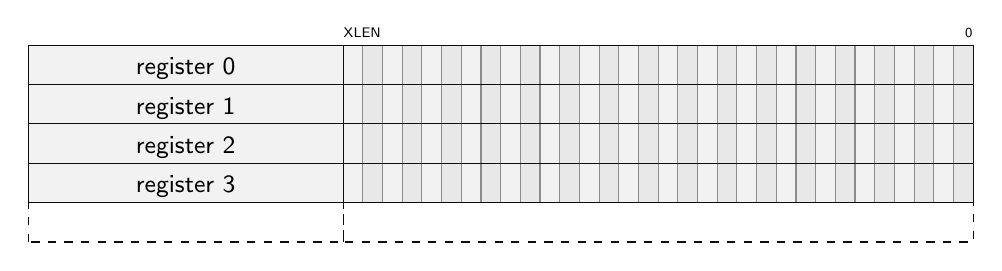
\begin{tikzpicture}[scale=0.5]
\begin{scope}[every node/.style={font=\small, inner sep=0pt, right}]

\foreach \x in {0,...,3}
  \fill [black!5] (0,\x)    rectangle (8,\x+1);
\foreach \x in {0,...,3}
  \draw [black!95] (0,\x)    rectangle (8,\x+1);
\foreach \x in {0,...,3} {
  \pgfmathsetmacro{\z}{int(3-\x)}
  \node [font=\small,anchor=base] at (4,\x+0.25)  {\textsf{register \z}};
}

\draw [black!95,dashed] (0,-1)      rectangle (8,0);

\foreach \x in {0,...,3}
  \draw [black!95] (8,\x)    rectangle (24,\x+1);
\foreach \x in {0,...,3} {
  \foreach \y in {0,4,...,60} {
    \fill [black!5]  (8+\y/4,\x)    rectangle (8.5+\y/4,\x+1);
    \draw [black!45] (8+\y/4,\x)    rectangle (8.5+\y/4,\x+1);
  }
  \foreach \y in {2,6,...,62} {
    \fill [black!9] (8+\y/4,\x)    rectangle (8.5+\y/4,\x+1);
    \draw [black!45] (8+\y/4,\x)    rectangle (8.5+\y/4,\x+1);
  }
  \draw [black!95] (8,\x) rectangle (24,\x+1);
}
\node [font=\tiny,anchor=base west] at (8,4.2)  {\textsf{XLEN}};
\node [font=\tiny,anchor=base east] at (24,4.2)  {\textsf{0}};

\draw [black!95,dashed] (8,-1)      rectangle (24,0);

\end{scope}
\end{tikzpicture}
\caption{organization of register storage.}
\label{fig:register-organization}
\end{figure}

\subsection{memory}

main memory is primary storage which in modern computers is most likely
\emph{DRAM}\footnote{\emph{DRAM}\,– Dynamic random-access memory.}.
main memory is organized as a byte-addressable store where each address
refers to a byte which is 8-bits of data. \emph{ALEN} is a parameter that
specifies the width of addresses in bits.
\\
\begin{figure}[H]
\centering
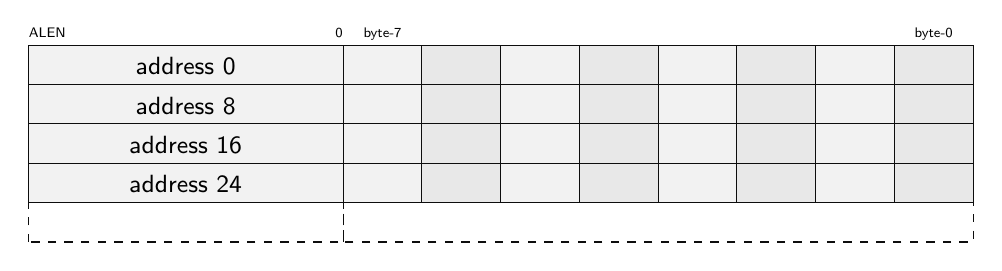
\begin{tikzpicture}[scale=0.5]
\begin{scope}[every node/.style={font=\small, inner sep=0pt, right}]

\foreach \x in {0,...,3}
  \fill [black!5] (0,\x)    rectangle (8,\x+1);
\foreach \x in {0,...,3}
  \draw [black!95] (0,\x)    rectangle (8,\x+1);
\foreach \x in {0,...,3} {
  \pgfmathsetmacro{\z}{int((3-\x)*8)}
  \node [font=\small,anchor=base] at (4,\x+0.25)  {\textsf{address \z}};
}
\node [font=\tiny,anchor=base west] at (0,4.2)  {\textsf{ALEN}};
\node [font=\tiny,anchor=base east] at (8,4.2)  {\textsf{0}};

\draw [black!95,dashed] (0,-1)      rectangle (8,0);

\foreach \x in {0,...,3} {
  \foreach \y in {0,2,...,6} {
    \fill [black!5] (8+\y*2,\x)     rectangle (10+\y*2,\x+1);
    \draw [black!95] (8+\y*2,\x)    rectangle (10+\y*2,\x+1);
  }
  \foreach \y in {1,3,...,7} {
    \fill [black!9] (8+\y*2,\x)    rectangle (10+\y*2,\x+1);
    \draw [black!95] (8+\y*2,\x)    rectangle (10+\y*2,\x+1);
  }
}
\node [font=\tiny,anchor=base] at (9,4.2)  {\textsf{byte-7}};
\node [font=\tiny,anchor=base] at (23,4.2)  {\textsf{byte-0}};

\draw [black!95,dashed] (8,-1)      rectangle (24,0);

\end{scope}
\end{tikzpicture}
\caption{organization of main-memory storage.}
\label{fig:main-memory-organization}
\end{figure}

\newpage
\subsection{instructions}
\label{sec:instructions}

instruction memory is a memory region dedicated to program instructions.
it is organized as a word-addressable store, similar to main memory,
but is read-only and reserved exclusively for instructions. this
configuration is typically referred to as a Harvard architecture%
~\cite{aiken1946marki}, in contrast to a Von Neumann architecture%
~\cite{vonneumann1945edvac,mauchly1946eniac}, which uses a shared
memory region for both program instructions and data.
\\
\par\noindent
instruction words contain packets of 16-bits which are composed of
size, opcode, and operand fields. instruction packets can be appended
together to form larger instruction words with larger opcode and
operand fields. section~\ref{sec:instruction-format} provides details
on the instruction template and instruction forms.
\\
\begin{figure}[H]
\centering
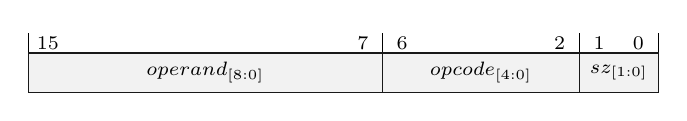
\begin{tikzpicture}[scale=0.5]
\node at (15.500000,1.250000) [font=\scriptsize] {1};
\node at (16.500000,1.250000) [font=\scriptsize] {0};
\node at (10.500000,1.250000) [font=\scriptsize] {6};
\node at (14.500000,1.250000) [font=\scriptsize] {2};
\node at (1.500000,1.250000) [font=\scriptsize] {15};
\node at (9.500000,1.250000) [font=\scriptsize] {7};
\draw (15.000000,1.000000) -- (15.000000,1.500000);
\draw (10.000000,1.000000) -- (10.000000,1.500000);
\draw (1.000000,1.000000) -- (1.000000,1.500000);
\draw (17.000000,1.000000) -- (17.000000,1.500000);
\fill [black!5]  (15.000000,0.000000) rectangle (17.000000,1.000000);
\draw [black!90]  (15.000000,0.000000) rectangle (17.000000,1.000000);
\node at (16.000000,0.500000) [font=\scriptsize] {$sz_{[1:0]}$};
\fill [black!5]  (10.000000,0.000000) rectangle (15.000000,1.000000);
\draw [black!90]  (10.000000,0.000000) rectangle (15.000000,1.000000);
\node at (12.500000,0.500000) [font=\scriptsize] {$opcode_{[4:0]}$};
\fill [black!5]  (1.000000,0.000000) rectangle (10.000000,1.000000);
\draw [black!90]  (1.000000,0.000000) rectangle (10.000000,1.000000);
\node at (5.500000,0.500000) [font=\scriptsize] {$operand_{[8:0]}$};
\end{tikzpicture}
\caption{16-bit instruction containing one packet.}
\label{fig:16-bit-instruction-word}
\end{figure}

\begin{figure}[H]
\centering
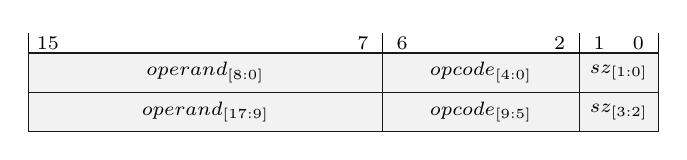
\begin{tikzpicture}[scale=0.5]
\node at (15.500000,1.250000) [font=\scriptsize] {1};
\node at (16.500000,1.250000) [font=\scriptsize] {0};
\node at (10.500000,1.250000) [font=\scriptsize] {6};
\node at (14.500000,1.250000) [font=\scriptsize] {2};
\node at (1.500000,1.250000) [font=\scriptsize] {15};
\node at (9.500000,1.250000) [font=\scriptsize] {7};
\draw (15.000000,1.000000) -- (15.000000,1.500000);
\draw (10.000000,1.000000) -- (10.000000,1.500000);
\draw (1.000000,1.000000) -- (1.000000,1.500000);
\draw (17.000000,1.000000) -- (17.000000,1.500000);
\fill [black!5]  (15.000000,0.000000) rectangle (17.000000,1.000000);
\draw [black!90]  (15.000000,0.000000) rectangle (17.000000,1.000000);
\node at (16.000000,0.500000) [font=\scriptsize] {$sz_{[1:0]}$};
\fill [black!5]  (10.000000,0.000000) rectangle (15.000000,1.000000);
\draw [black!90]  (10.000000,0.000000) rectangle (15.000000,1.000000);
\node at (12.500000,0.500000) [font=\scriptsize] {$opcode_{[4:0]}$};
\fill [black!5]  (1.000000,0.000000) rectangle (10.000000,1.000000);
\draw [black!90]  (1.000000,0.000000) rectangle (10.000000,1.000000);
\node at (5.500000,0.500000) [font=\scriptsize] {$operand_{[8:0]}$};
\fill [black!5]  (15.000000,-1.000000) rectangle (17.000000,0.000000);
\draw [black!90]  (15.000000,-1.000000) rectangle (17.000000,0.000000);
\node at (16.000000,-0.500000) [font=\scriptsize] {$sz_{[3:2]}$};
\fill [black!5]  (10.000000,-1.000000) rectangle (15.000000,0.000000);
\draw [black!90]  (10.000000,-1.000000) rectangle (15.000000,0.000000);
\node at (12.500000,-0.500000) [font=\scriptsize] {$opcode_{[9:5]}$};
\fill [black!5]  (1.000000,-1.000000) rectangle (10.000000,0.000000);
\draw [black!90]  (1.000000,-1.000000) rectangle (10.000000,0.000000);
\node at (5.500000,-0.500000) [font=\scriptsize] {$operand_{[17:9]}$};
\end{tikzpicture}
\caption{32-bit instruction containing two packets.}
\label{fig:32-bit-instruction-word}
\end{figure}

\par\noindent
instruction words are packed together into instruction blocks
containing instruction size information that is used to fuse
them together to compose variable-length instructions~\cite{US5717881A}.
instruction words can begin on any 16-bit aligned address.
instruction memory is addressed with displacements from the \emph{program
counter} called \emph{pc-relative} addresses.
\\
\begin{figure}[H]
\centering
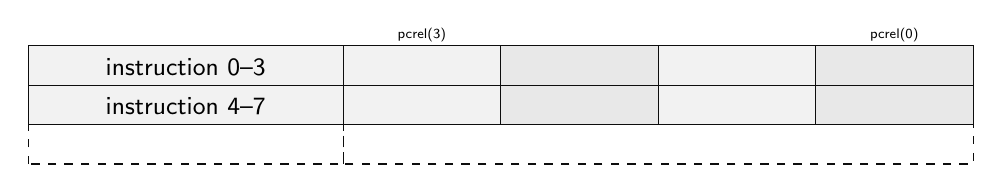
\begin{tikzpicture}[scale=0.5]
\begin{scope}[every node/.style={font=\small, inner sep=0pt, right}]
\foreach \x in {0,...,1} {
  \fill [black!5] (0,\x)    rectangle (8,\x+1);
  \draw [black!95] (0,\x)    rectangle (8,\x+1);
  \pgfmathsetmacro{\y}{int((1-\x)*4)}
  \pgfmathsetmacro{\z}{int((1-\x)*4+3)}
  \node [font=\small,anchor=base] at (4,\x+0.25)  {\textsf{instruction \y--\z}};
  \foreach \y in {0,2} {
    \fill [black!5]  (8+\y*4,\x)    rectangle (12+\y*4,\x+1);
    \draw [black!95] (8+\y*4,\x)    rectangle (12+\y*4,\x+1);
  }
  \foreach \y in {1,3} {
    \fill [black!9]  (8+\y*4,\x)    rectangle (12+\y*4,\x+1);
    \draw [black!95] (8+\y*4,\x)    rectangle (12+\y*4,\x+1);
  }
}
\draw [black!95,dashed] (0,-1)      rectangle (8,0);
\draw [black!95,dashed] (8,-1)      rectangle (24,0);
\node [font=\tiny,anchor=base] at (10,2.2)  {\textsf{pcrel(3)}};
\node [font=\tiny,anchor=base] at (22,2.2)  {\textsf{pcrel(0)}};
\end{scope}
\end{tikzpicture}
\caption{organization of instruction-memory with 16-bit instructions.}
\label{fig:instruction-memory-16}
\end{figure}

\begin{figure}[H]
\centering
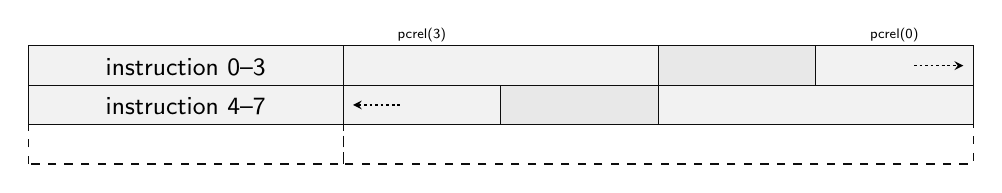
\begin{tikzpicture}[scale=0.5]
\begin{scope}[every node/.style={font=\small, inner sep=0pt, right}]

\fill [black!5] (0,0)    rectangle (8,1);
\draw [black!95] (0,0)    rectangle (8,1);
\node [font=\small,anchor=base] at (4,0.25)  {\textsf{instruction 4--7}};
\fill [black!5] (8,0)    rectangle (12,1);
\fill [black!9] (12,0)    rectangle (16,1);
\fill [black!5] (16,0)    rectangle (24,1);
\draw [black!95] (8,0)    rectangle (12,1);
\draw [black!95] (12,0)    rectangle (16,1);
\draw [black!95] (16,0)    rectangle (24,1);
\draw[<-, >=stealth, dash pattern=on 1pt off 1pt] (8.25,0.5) -- (9.5,0.5);

\fill [black!5] (0,1)    rectangle (8,2);
\draw [black!95] (0,1)    rectangle (8,2);
\node [font=\small,anchor=base] at (4,1.25)  {\textsf{instruction 0--3}};
\fill [black!5] (8,1)    rectangle (16,2);
\fill [black!9] (16,1)    rectangle (20,2);
\fill [black!5] (20,1)    rectangle (24,2);
\draw [black!95] (8,1)    rectangle (16,2);
\draw [black!95] (16,1)    rectangle (20,2);
\draw [black!95] (20,1)    rectangle (24,2);
\draw[->, >=stealth, dash pattern=on 1pt off 1pt] (22.5,1.5) -- (23.75,1.5);

\draw [black!95,dashed] (0,-1)      rectangle (8,0);
\draw [black!95,dashed] (8,-1)      rectangle (24,0);
\node [font=\tiny,anchor=base] at (10,2.2)  {\textsf{pcrel(3)}};
\node [font=\tiny,anchor=base] at (22,2.2)  {\textsf{pcrel(0)}};
\end{scope}
\end{tikzpicture}
\caption{organization of instruction-memory with 16-bit and 32-bit instructions.}
\label{fig:instruction-memory-16-32}
\end{figure}

\newpage
\subsection{constants}
\label{sec:constants}

constant memory~\cite{Solomonoff1964} is a memory region dedicated to
constants. it is organized as a word-addressable store like main-memory,
but is read-only and restricted to constants. instructions can refer to
constants using \emph{ib-relative} addresses inside instruction operands.
section~\ref{sec:program-streams} provides more details on the split
instruction and constant streams.
\\
\par\noindent
constant memory is addressed with displacements from the \emph{immediate
base} register called \emph{ib-relative} addresses which are stored inside
instruction operand slots, are sized, scaled and aligned addresses computed
relative to the \emph{immediate base} register, which is like a program
counter for constants. these diagrams show $ib8(n)$ through $ib64(n)$
\emph{ib-relative} addresses for access to 8-bit through to 64-bit constants
respectively: \emph{note: ib-relative addresses alias a single constant
storage space containing all types.}
\\
\begin{figure}[H]
\centering
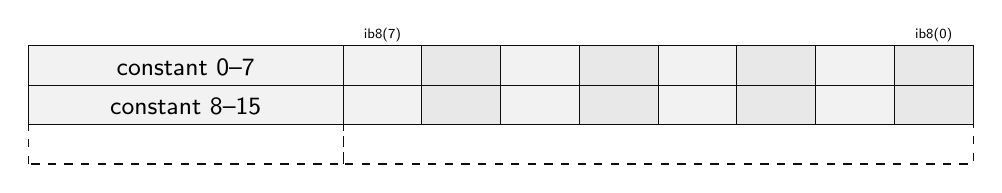
\begin{tikzpicture}[scale=0.5]
\begin{scope}[every node/.style={font=\small, inner sep=0pt, right}]
\foreach \x in {0,...,1} {
  \fill [black!5] (0,\x)    rectangle (8,\x+1);
  \draw [black!95] (0,\x)    rectangle (8,\x+1);
  \pgfmathsetmacro{\y}{int((1-\x)*8)}
  \pgfmathsetmacro{\z}{int((1-\x)*8+7)}
  \node [font=\small,anchor=base] at (4,\x+0.25)  {\textsf{constant \y--\z}};
  \foreach \y in {0,2,...,6} {
    \fill [black!5]  (8+\y*2,\x)    rectangle (10+\y*2,\x+1);
    \draw [black!95] (8+\y*2,\x)    rectangle (10+\y*2,\x+1);
  }
  \foreach \y in {1,3,...,7} {
    \fill [black!9]  (8+\y*2,\x)    rectangle (10+\y*2,\x+1);
    \draw [black!95] (8+\y*2,\x)    rectangle (10+\y*2,\x+1);
  }
}
\draw [black!95,dashed] (0,-1)      rectangle (8,0);
\draw [black!95,dashed] (8,-1)      rectangle (24,0);
\node [font=\tiny,anchor=base] at (9,2.2)  {\textsf{ib8(7)}};
\node [font=\tiny,anchor=base] at (23,2.2)  {\textsf{ib8(0)}};
\end{scope}
\end{tikzpicture}
\caption{organization of \emph{ib8} constant-memory storage.}
\label{fig:constant-memory-ib8-organization}
\end{figure}

\begin{figure}[H]
\centering
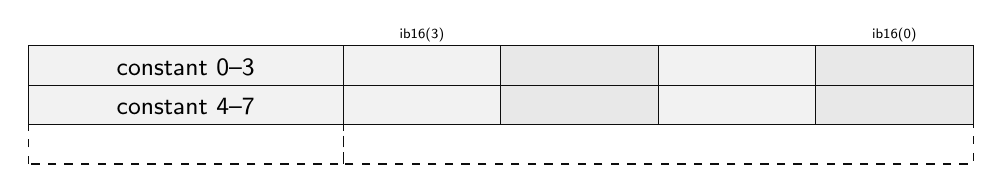
\begin{tikzpicture}[scale=0.5]
\begin{scope}[every node/.style={font=\small, inner sep=0pt, right}]
\foreach \x in {0,...,1} {
  \fill [black!5] (0,\x)    rectangle (8,\x+1);
  \draw [black!95] (0,\x)    rectangle (8,\x+1);
  \pgfmathsetmacro{\y}{int((1-\x)*4)}
  \pgfmathsetmacro{\z}{int((1-\x)*4+3)}
  \node [font=\small,anchor=base] at (4,\x+0.25)  {\textsf{constant \y--\z}};
  \foreach \y in {0,2} {
    \fill [black!5]  (8+\y*4,\x)    rectangle (12+\y*4,\x+1);
    \draw [black!95] (8+\y*4,\x)    rectangle (12+\y*4,\x+1);
  }
  \foreach \y in {1,3} {
    \fill [black!9]  (8+\y*4,\x)    rectangle (12+\y*4,\x+1);
    \draw [black!95] (8+\y*4,\x)    rectangle (12+\y*4,\x+1);
  }
}
\draw [black!95,dashed] (0,-1)      rectangle (8,0);
\draw [black!95,dashed] (8,-1)      rectangle (24,0);
\node [font=\tiny,anchor=base] at (10,2.2)  {\textsf{ib16(3)}};
\node [font=\tiny,anchor=base] at (22,2.2)  {\textsf{ib16(0)}};
\end{scope}
\end{tikzpicture}
\caption{organization of \emph{ib16} constant-memory storage.}
\label{fig:constant-memory-ib16-organization}
\end{figure}

\begin{figure}[H]
\centering
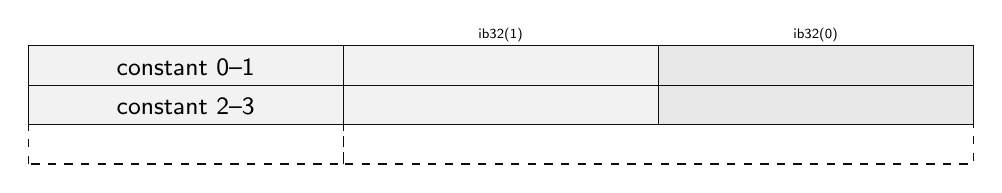
\begin{tikzpicture}[scale=0.5]
\begin{scope}[every node/.style={font=\small, inner sep=0pt, right}]
\foreach \x in {0,...,1} {
  \fill [black!5] (0,\x)    rectangle (8,\x+1);
  \draw [black!95] (0,\x)    rectangle (8,\x+1);
  \pgfmathsetmacro{\y}{int((1-\x)*2)}
  \pgfmathsetmacro{\z}{int((1-\x)*2+1)}
  \node [font=\small,anchor=base] at (4,\x+0.25)  {\textsf{constant \y--\z}};
  \foreach \y in {0} {
    \fill [black!5]  (8+\y*8,\x)    rectangle (16+\y*8,\x+1);
    \draw [black!95] (8+\y*8,\x)    rectangle (16+\y*8,\x+1);
  }
  \foreach \y in {1} {
    \fill [black!9]  (8+\y*8,\x)    rectangle (16+\y*8,\x+1);
    \draw [black!95] (8+\y*8,\x)    rectangle (16+\y*8,\x+1);
  }
}
\draw [black!95,dashed] (0,-1)      rectangle (8,0);
\draw [black!95,dashed] (8,-1)      rectangle (24,0);
\node [font=\tiny,anchor=base] at (12,2.2)  {\textsf{ib32(1)}};
\node [font=\tiny,anchor=base] at (20,2.2)  {\textsf{ib32(0)}};
\end{scope}
\end{tikzpicture}
\caption{organization of \emph{ib32} constant-memory storage.}
\label{fig:constant-memory-ib32-organization}
\end{figure}

\begin{figure}[H]
\centering
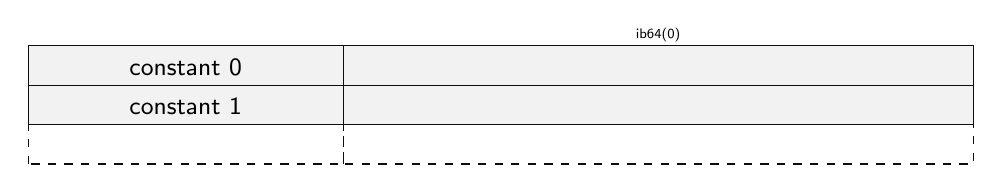
\begin{tikzpicture}[scale=0.5]
\begin{scope}[every node/.style={font=\small, inner sep=0pt, right}]
\foreach \x in {0,...,1} {
  \fill [black!5] (0,\x)    rectangle (8,\x+1);
  \draw [black!95] (0,\x)    rectangle (8,\x+1);
  \pgfmathsetmacro{\y}{int(1-\x)}
  \node [font=\small,anchor=base] at (4,\x+0.25)  {\textsf{constant \y}};
  \fill [black!5] (8,\x)    rectangle (24,\x+1);
  \foreach \y in {0,...,0} {
    \draw [black!95] (8+\y*16,\x)    rectangle (24+\y*16,\x+1);
  }
}
\draw [black!95,dashed] (0,-1)      rectangle (8,0);
\draw [black!95,dashed] (8,-1)      rectangle (24,0);
\node [font=\tiny,anchor=base] at (16,2.2)  {\textsf{ib64(0)}};
\end{scope}
\end{tikzpicture}
\caption{organization of \emph{ib64} constant-memory storage.}
\label{fig:constant-memory-ib64-organization}
\end{figure}

\newpage
\section{Core concepts}

\par\noindent
glyph is a super regular RISC architecture that encodes constants in a
secondary stream accessed via an \emph{immediate base} register that points at
immediate blocks containing constants accessed via a constant address
mode. the \emph{immediate base} register branches like the
\emph{program counter}, and procedure calls and returns set and restore
\emph{(pc,ib)} together.
\\
\par\noindent
glyph uses relative address vectors in its link register which is different
to typical RISC architectures. glyph does this so that the branch instructions
can fit \emph{(pc,ib)} into the a single link register for compatibility with
traditional RISC architectures. glyph achieves this by packing two relative
\emph{(pc,ib)} displacements into a relative address vector\footnote{the
architecture defines two parameters: \emph{ALEN} and \emph{XLEN},
which respectively to refer to width of addresses and width of general
purpose registers in bits. when $XLEN \ge ALEN \times 2$ it is possible to
pack absolute addresses instead of relative addresses, as would be the case
where \emph{ALEN=64} and \emph{XLEN=128}.}.
\\
\par\noindent
immediate blocks can be switched using the immediate block branch
instruction. immediate blocks, unlike typical RISC architectures, mean
that most relocations are word sized like CISC architectures, and can
use C-style structure packing and alignment rules.
\\
\par\noindent
this list outlines some differentiating elements of the super regular
RISC architecture:

\begin{itemize}[itemsep=0pt]
\item variable length instruction format supporting 16, 32, 64, and 128-bit
instructions.
\item 16-bit compressed instruction packets can access 8 registers.
\item \emph{(pc,ib)} is a \emph{program counter} and
\emph{immediate base} register address vector.
\item link register contains a packed relative \emph{(pc,ib)} address vector
to function entry.
\item \texttt{ibj} \emph{immediate-block-jump} adds a relative address to
the \emph{immediate base} register.
\item \texttt{movw} \emph{move-word-immediate-block} uses an unsigned
displacement to access constants.
\item \texttt{jalib} \emph{jump-and-link-immediate-block} or \emph{call}
\emph{link function}
links address vector and adds constants to \emph{(pc,ib)} and is used
to branch the \emph{program counter} and \emph{immediate base} register
at the same time for calling procedures.
\item \texttt{jtlib} \emph{jump-to-link-immediate-block} or \emph{return}
\emph{link function}
subtracts link vector from and adds constants to \emph{(pc,ib)} and is
used to branch the \emph{program counter} and \emph{immediate base}
register at the same time for returning from called procedures.
\item \texttt{pin} \emph{pack-indirect} packs two absolute addresses as
relative address vector from \emph{(pc,ib)} and is used for calling
absolute addresses such as virtual functions.
\end{itemize}

\par\noindent
the \texttt{pin} and \texttt{link} instructions form a modular arithmetic
ring of relative address vectors, due to their use of relative addresses.
relative address vectors can be encrypted, decrypted, and authenticated to
form a verifiable chain of addresses for control flow integrity.

\newpage
\section{Program streams}
\label{sec:program-streams}

glyph seperates the stored programs into two streams, one with instructions
and one with constants~\cite{Solomonoff1964}. the instruction stream is
addressed with the \emph{program counter (pc)} and the constant stream is
addressed with the \emph{immediate base (ib)} register. this could be
referred to as split program stream Harvard architecture.

\begin{figure}[H]
\centering
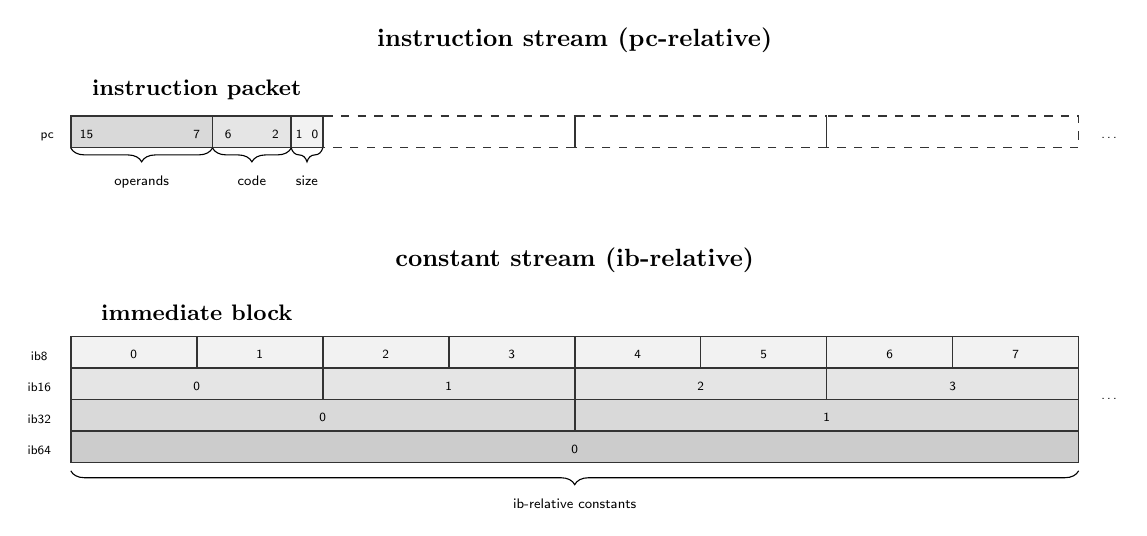
\begin{tikzpicture}[scale=0.4]
\begin{scope}[every node/.style={font=\normalsize, inner sep=0pt, right}]

\node [above,scale=0.9,anchor=south] at (16,3)  {\textbf{instruction stream (pc-relative)}};
\node [font=\small,above,scale=0.9,anchor=south] at (4,1.5)  {\textbf{instruction packet}};
\node [font=\tiny,below,scale=0.9,anchor=base] at (-0.75,0.3)  {\textsf{pc}};
\node [font=\tiny,below,scale=0.9,anchor=base] at (33.0,0.3)  {\textsf{\ldots}};

\fill [black!15]                   (0.0,0.0)   rectangle (4.5,1.0);
\draw [line width=0.2mm, black!80] (0.0,0.0)   rectangle (4.5,1.0);
\node [font=\tiny,below,scale=0.9,anchor=base] at (0.5,0.3)  {\textsf{15}};
\node [font=\tiny,below,scale=0.9,anchor=base] at (4.0,0.3)  {\textsf{7}};

\fill [black!10]                   (4.5,0.0)   rectangle (7.0,1.0);
\draw [line width=0.2mm, black!80] (4.5,0.0)   rectangle (7.0,1.0);
\node [font=\tiny,below,scale=0.9,anchor=base] at (5.0,0.3)  {\textsf{6}};
\node [font=\tiny,below,scale=0.9,anchor=base] at (6.5,0.3)  {\textsf{2}};

\fill [black!5]                    (7.0,0.0)   rectangle (8.0,1.0);
\draw [line width=0.2mm, black!80] (7.0,0,0)   rectangle (8.0,1.0);
\node [font=\tiny,below,scale=0.9,anchor=base] at (7.25,0.3)  {\textsf{1}};
\node [font=\tiny,below,scale=0.9,anchor=base] at (7.75,0.3)  {\textsf{0}};

\draw [line width=0.2mm, black!80,dashed] (8,0)      rectangle (16,1);
\draw [line width=0.2mm, black!80,dashed] (16,0)     rectangle (24,1);
\draw [line width=0.2mm, black!80,dashed] (24,0)     rectangle (32,1);

\draw [decorate,decoration={brace,amplitude=5pt,mirror,raise=4ex}]
    (0,1.5) -- (4.5,1.5) node[font=\tiny,midway,below,yshift=-2.7em]{\textsf{operands}};

\draw [decorate,decoration={brace,amplitude=5pt,mirror,raise=4ex}]
    (4.5,1.5) -- (7,1.5) node[font=\tiny,midway,below,yshift=-2.7em]{\textsf{code}};

\draw [decorate,decoration={brace,amplitude=5pt,mirror,raise=4ex}]
    (7,1.5) -- (8,1.5) node[font=\tiny,midway,below,yshift=-2.7em]{\textsf{size}};

\node [above,scale=0.9,anchor=south] at (16,-4)  {\textbf{constant stream (ib-relative)}};
\node [font=\small,above,scale=0.9,anchor=south] at (4,-5.5)  {\textbf{immediate block}};

\node [font=\tiny,below,scale=0.9,anchor=base] at (33.0,-8.0)  {\textsf{\ldots}};

\node [font=\tiny,below,scale=0.9,anchor=base] at (-1.0,-6.75)  {\textsf{ib8}};
\foreach \x in {0,1,2,3,4,5,6,7}
  \fill [black!5]                   (\x*4,-6)     rectangle (\x*4+4,-7);
\foreach \x in {0,1,2,3,4,5,6,7}
  \draw [line width=0.2mm, black!80] (\x*4,-6)     rectangle (\x*4+4,-7);
\foreach \x in {0,1,2,3,4,5,6,7}
  \node [font=\tiny,below,scale=0.9,anchor=base] at (\x*4 + 2,-6.7)  {\textsf{\x}};

\node [font=\tiny,below,scale=0.9,anchor=base] at (-1.0,-7.75)  {\textsf{ib16}};
\foreach \x in {0,1,2,3}
  \fill [black!10]                   (\x*8,-7)     rectangle (\x*8+8,-8);
\foreach \x in {0,1,2,3}
  \draw [line width=0.2mm, black!80] (\x*8,-7)     rectangle (\x*8+8,-8);
\foreach \x in {0,1,2,3}
  \node [font=\tiny,below,scale=0.9,anchor=base] at (\x*8 + 4,-7.7)  {\textsf{\x}};

\node [font=\tiny,below,scale=0.9,anchor=base] at (-1.0,-8.75)  {\textsf{ib32}};
\foreach \x in {0,1}
  \fill [black!15]                   (\x*16,-8)     rectangle (\x*16+16,-9);
\foreach \x in {0,1}
  \draw [line width=0.2mm, black!80] (\x*16,-8)     rectangle (\x*16+16,-9);
\foreach \x in {0,1}
  \node [font=\tiny,below,scale=0.9,anchor=base] at (\x*16 + 8,-8.7)  {\textsf{\x}};

\node [font=\tiny,below,scale=0.9,anchor=base] at (-1.0,-9.75)  {\textsf{ib64}};
\foreach \x in {0}
  \fill [black!20]                   (\x*32,-9)     rectangle (\x*32+32,-10);
\foreach \x in {0}
  \draw [line width=0.2mm, black!80] (\x*32,-9)     rectangle (\x*32+32,-10);
\foreach \x in {0}
  \node [font=\tiny,below,scale=0.9,anchor=base] at (\x*32 + 16,-9.7)  {\textsf{\x}};

\draw [decorate,decoration={brace,amplitude=5pt,mirror,raise=4ex}]
    (0,-8.75) -- (32,-8.75) node[font=\tiny,midway,below,yshift=-2.7em]
        {\textsf{ib-relative constants}};

\end{scope}
\end{tikzpicture}
\caption{program counter and immediate base register.}
\label{fig:glyph-program-streams}
\end{figure}

\par\noindent
instruction blocks are aligned memory blocks addressed by the \emph{program
counter}. instruction memory is addressed with \emph{pc-relative} addresses
in instruction immediate values or indirectly with constants accessed using
\emph{ib-relative} addresses stored inside instruction operand slots.
\\
\par\noindent
immediate blocks are aligned memory blocks addressed by the \emph{immediate
base} register. constant memory is addressed with \emph{ib-relative}
addresses stored inside instruction operand slots, which are sized, scaled,
and aligned relative to the \emph{immediate base} register.
\\
\par\noindent
the constant stream branches independently using the
\emph{immediate-block-jump} instruction to update the \emph{immediate base}
register, or together with the \emph{program counter} in procedure call and
return instructions that branch instruction and constants at the same time;
\emph{jump-and-link-immediate-block} and \emph{jump-to-link-immediate-block}
add and subtract address vectors to \emph{(pc,ib)}. the \emph{pack-indirect}
instruction allows absolute \emph{(pc,ib)} addresses to be packed into an
address vector for indirect calls.
\\
\par\noindent
the instruction forms use bonded operand slots for immediate operands and
operand bits do not overlap opcode bits. the use of immediate blocks means
large immediate constants can all be accessed using short references encoded
inside of operand slots for instructions that use an immediate block
relative addressing mode.
\\

\newpage
\section{Instruction format}
\label{sec:instruction-format}

instructions use a variable length format~\cite{US5717881A} with a
16-bit instruction packet that supports 16, 32, 64, and 128-bit
instruction words. the instruction packet uses a \emph{super regular}
scheme, whereby successive instruction packets extend the fields in
the previous instruction packet~\cite{US6877084B1}. instruction words
can begin on any 16-bit aligned address.

\subsection{instruction templates}

the variable length instruction format has a single base format
where fields in the template instruction form are extended by
successive instruction packets.

\begin{figure}[H]
\centering
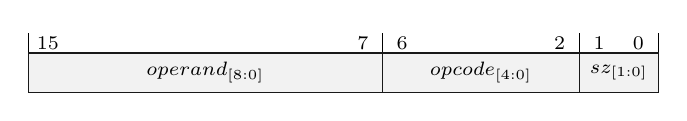
\begin{tikzpicture}[scale=0.5]
\node at (15.500000,1.250000) [font=\scriptsize] {1};
\node at (16.500000,1.250000) [font=\scriptsize] {0};
\node at (10.500000,1.250000) [font=\scriptsize] {6};
\node at (14.500000,1.250000) [font=\scriptsize] {2};
\node at (1.500000,1.250000) [font=\scriptsize] {15};
\node at (9.500000,1.250000) [font=\scriptsize] {7};
\draw (15.000000,1.000000) -- (15.000000,1.500000);
\draw (10.000000,1.000000) -- (10.000000,1.500000);
\draw (1.000000,1.000000) -- (1.000000,1.500000);
\draw (17.000000,1.000000) -- (17.000000,1.500000);
\fill [black!5]  (15.000000,0.000000) rectangle (17.000000,1.000000);
\draw [black!90]  (15.000000,0.000000) rectangle (17.000000,1.000000);
\node at (16.000000,0.500000) [font=\scriptsize] {$sz_{[1:0]}$};
\fill [black!5]  (10.000000,0.000000) rectangle (15.000000,1.000000);
\draw [black!90]  (10.000000,0.000000) rectangle (15.000000,1.000000);
\node at (12.500000,0.500000) [font=\scriptsize] {$opcode_{[4:0]}$};
\fill [black!5]  (1.000000,0.000000) rectangle (10.000000,1.000000);
\draw [black!90]  (1.000000,0.000000) rectangle (10.000000,1.000000);
\node at (5.500000,0.500000) [font=\scriptsize] {$operand_{[8:0]}$};
\end{tikzpicture}
\caption{instruction template --- 16-bit.}
\label{fig:glyph-instruction-template-16}
\end{figure}

\begin{figure}[H]
\centering
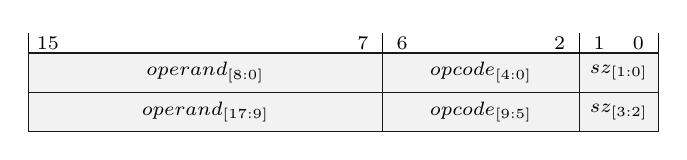
\begin{tikzpicture}[scale=0.5]
\node at (15.500000,1.250000) [font=\scriptsize] {1};
\node at (16.500000,1.250000) [font=\scriptsize] {0};
\node at (10.500000,1.250000) [font=\scriptsize] {6};
\node at (14.500000,1.250000) [font=\scriptsize] {2};
\node at (1.500000,1.250000) [font=\scriptsize] {15};
\node at (9.500000,1.250000) [font=\scriptsize] {7};
\draw (15.000000,1.000000) -- (15.000000,1.500000);
\draw (10.000000,1.000000) -- (10.000000,1.500000);
\draw (1.000000,1.000000) -- (1.000000,1.500000);
\draw (17.000000,1.000000) -- (17.000000,1.500000);
\fill [black!5]  (15.000000,0.000000) rectangle (17.000000,1.000000);
\draw [black!90]  (15.000000,0.000000) rectangle (17.000000,1.000000);
\node at (16.000000,0.500000) [font=\scriptsize] {$sz_{[1:0]}$};
\fill [black!5]  (10.000000,0.000000) rectangle (15.000000,1.000000);
\draw [black!90]  (10.000000,0.000000) rectangle (15.000000,1.000000);
\node at (12.500000,0.500000) [font=\scriptsize] {$opcode_{[4:0]}$};
\fill [black!5]  (1.000000,0.000000) rectangle (10.000000,1.000000);
\draw [black!90]  (1.000000,0.000000) rectangle (10.000000,1.000000);
\node at (5.500000,0.500000) [font=\scriptsize] {$operand_{[8:0]}$};
\fill [black!5]  (15.000000,-1.000000) rectangle (17.000000,0.000000);
\draw [black!90]  (15.000000,-1.000000) rectangle (17.000000,0.000000);
\node at (16.000000,-0.500000) [font=\scriptsize] {$sz_{[3:2]}$};
\fill [black!5]  (10.000000,-1.000000) rectangle (15.000000,0.000000);
\draw [black!90]  (10.000000,-1.000000) rectangle (15.000000,0.000000);
\node at (12.500000,-0.500000) [font=\scriptsize] {$opcode_{[9:5]}$};
\fill [black!5]  (1.000000,-1.000000) rectangle (10.000000,0.000000);
\draw [black!90]  (1.000000,-1.000000) rectangle (10.000000,0.000000);
\node at (5.500000,-0.500000) [font=\scriptsize] {$operand_{[17:9]}$};
\end{tikzpicture}
\caption{instruction template --- 32-bit.}
\label{fig:glyph-instruction-template-32}
\end{figure}

\begin{figure}[H]
\centering
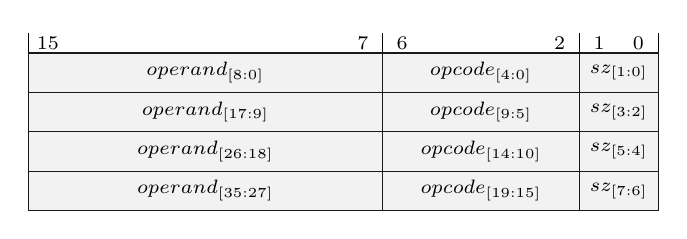
\begin{tikzpicture}[scale=0.5]
\node at (15.500000,1.250000) [font=\scriptsize] {1};
\node at (16.500000,1.250000) [font=\scriptsize] {0};
\node at (10.500000,1.250000) [font=\scriptsize] {6};
\node at (14.500000,1.250000) [font=\scriptsize] {2};
\node at (1.500000,1.250000) [font=\scriptsize] {15};
\node at (9.500000,1.250000) [font=\scriptsize] {7};
\draw (15.000000,1.000000) -- (15.000000,1.500000);
\draw (10.000000,1.000000) -- (10.000000,1.500000);
\draw (1.000000,1.000000) -- (1.000000,1.500000);
\draw (17.000000,1.000000) -- (17.000000,1.500000);
\fill [black!5]  (15.000000,0.000000) rectangle (17.000000,1.000000);
\draw [black!90]  (15.000000,0.000000) rectangle (17.000000,1.000000);
\node at (16.000000,0.500000) [font=\scriptsize] {$sz_{[1:0]}$};
\fill [black!5]  (10.000000,0.000000) rectangle (15.000000,1.000000);
\draw [black!90]  (10.000000,0.000000) rectangle (15.000000,1.000000);
\node at (12.500000,0.500000) [font=\scriptsize] {$opcode_{[4:0]}$};
\fill [black!5]  (1.000000,0.000000) rectangle (10.000000,1.000000);
\draw [black!90]  (1.000000,0.000000) rectangle (10.000000,1.000000);
\node at (5.500000,0.500000) [font=\scriptsize] {$operand_{[8:0]}$};
\fill [black!5]  (15.000000,-1.000000) rectangle (17.000000,0.000000);
\draw [black!90]  (15.000000,-1.000000) rectangle (17.000000,0.000000);
\node at (16.000000,-0.500000) [font=\scriptsize] {$sz_{[3:2]}$};
\fill [black!5]  (10.000000,-1.000000) rectangle (15.000000,0.000000);
\draw [black!90]  (10.000000,-1.000000) rectangle (15.000000,0.000000);
\node at (12.500000,-0.500000) [font=\scriptsize] {$opcode_{[9:5]}$};
\fill [black!5]  (1.000000,-1.000000) rectangle (10.000000,0.000000);
\draw [black!90]  (1.000000,-1.000000) rectangle (10.000000,0.000000);
\node at (5.500000,-0.500000) [font=\scriptsize] {$operand_{[17:9]}$};
\fill [black!5]  (15.000000,-2.000000) rectangle (17.000000,-1.000000);
\draw [black!90]  (15.000000,-2.000000) rectangle (17.000000,-1.000000);
\node at (16.000000,-1.500000) [font=\scriptsize] {$sz_{[5:4]}$};
\fill [black!5]  (10.000000,-2.000000) rectangle (15.000000,-1.000000);
\draw [black!90]  (10.000000,-2.000000) rectangle (15.000000,-1.000000);
\node at (12.500000,-1.500000) [font=\scriptsize] {$opcode_{[14:10]}$};
\fill [black!5]  (1.000000,-2.000000) rectangle (10.000000,-1.000000);
\draw [black!90]  (1.000000,-2.000000) rectangle (10.000000,-1.000000);
\node at (5.500000,-1.500000) [font=\scriptsize] {$operand_{[26:18]}$};
\fill [black!5]  (15.000000,-3.000000) rectangle (17.000000,-2.000000);
\draw [black!90]  (15.000000,-3.000000) rectangle (17.000000,-2.000000);
\node at (16.000000,-2.500000) [font=\scriptsize] {$sz_{[7:6]}$};
\fill [black!5]  (10.000000,-3.000000) rectangle (15.000000,-2.000000);
\draw [black!90]  (10.000000,-3.000000) rectangle (15.000000,-2.000000);
\node at (12.500000,-2.500000) [font=\scriptsize] {$opcode_{[19:15]}$};
\fill [black!5]  (1.000000,-3.000000) rectangle (10.000000,-2.000000);
\draw [black!90]  (1.000000,-3.000000) rectangle (10.000000,-2.000000);
\node at (5.500000,-2.500000) [font=\scriptsize] {$operand_{[35:27]}$};
\end{tikzpicture}
\caption{instruction template --- 64-bit.}
\label{fig:glyph-instruction-template-64}
\end{figure}

\begin{figure}[H]
\centering
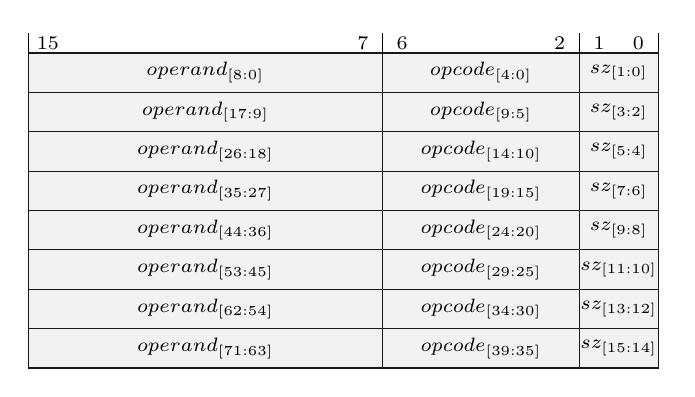
\begin{tikzpicture}[scale=0.5]
\node at (15.500000,1.250000) [font=\scriptsize] {1};
\node at (16.500000,1.250000) [font=\scriptsize] {0};
\node at (10.500000,1.250000) [font=\scriptsize] {6};
\node at (14.500000,1.250000) [font=\scriptsize] {2};
\node at (1.500000,1.250000) [font=\scriptsize] {15};
\node at (9.500000,1.250000) [font=\scriptsize] {7};
\draw (15.000000,1.000000) -- (15.000000,1.500000);
\draw (10.000000,1.000000) -- (10.000000,1.500000);
\draw (1.000000,1.000000) -- (1.000000,1.500000);
\draw (17.000000,1.000000) -- (17.000000,1.500000);
\fill [black!5]  (15.000000,0.000000) rectangle (17.000000,1.000000);
\draw [black!90]  (15.000000,0.000000) rectangle (17.000000,1.000000);
\node at (16.000000,0.500000) [font=\scriptsize] {$sz_{[1:0]}$};
\fill [black!5]  (10.000000,0.000000) rectangle (15.000000,1.000000);
\draw [black!90]  (10.000000,0.000000) rectangle (15.000000,1.000000);
\node at (12.500000,0.500000) [font=\scriptsize] {$opcode_{[4:0]}$};
\fill [black!5]  (1.000000,0.000000) rectangle (10.000000,1.000000);
\draw [black!90]  (1.000000,0.000000) rectangle (10.000000,1.000000);
\node at (5.500000,0.500000) [font=\scriptsize] {$operand_{[8:0]}$};
\fill [black!5]  (15.000000,-1.000000) rectangle (17.000000,0.000000);
\draw [black!90]  (15.000000,-1.000000) rectangle (17.000000,0.000000);
\node at (16.000000,-0.500000) [font=\scriptsize] {$sz_{[3:2]}$};
\fill [black!5]  (10.000000,-1.000000) rectangle (15.000000,0.000000);
\draw [black!90]  (10.000000,-1.000000) rectangle (15.000000,0.000000);
\node at (12.500000,-0.500000) [font=\scriptsize] {$opcode_{[9:5]}$};
\fill [black!5]  (1.000000,-1.000000) rectangle (10.000000,0.000000);
\draw [black!90]  (1.000000,-1.000000) rectangle (10.000000,0.000000);
\node at (5.500000,-0.500000) [font=\scriptsize] {$operand_{[17:9]}$};
\fill [black!5]  (15.000000,-2.000000) rectangle (17.000000,-1.000000);
\draw [black!90]  (15.000000,-2.000000) rectangle (17.000000,-1.000000);
\node at (16.000000,-1.500000) [font=\scriptsize] {$sz_{[5:4]}$};
\fill [black!5]  (10.000000,-2.000000) rectangle (15.000000,-1.000000);
\draw [black!90]  (10.000000,-2.000000) rectangle (15.000000,-1.000000);
\node at (12.500000,-1.500000) [font=\scriptsize] {$opcode_{[14:10]}$};
\fill [black!5]  (1.000000,-2.000000) rectangle (10.000000,-1.000000);
\draw [black!90]  (1.000000,-2.000000) rectangle (10.000000,-1.000000);
\node at (5.500000,-1.500000) [font=\scriptsize] {$operand_{[26:18]}$};
\fill [black!5]  (15.000000,-3.000000) rectangle (17.000000,-2.000000);
\draw [black!90]  (15.000000,-3.000000) rectangle (17.000000,-2.000000);
\node at (16.000000,-2.500000) [font=\scriptsize] {$sz_{[7:6]}$};
\fill [black!5]  (10.000000,-3.000000) rectangle (15.000000,-2.000000);
\draw [black!90]  (10.000000,-3.000000) rectangle (15.000000,-2.000000);
\node at (12.500000,-2.500000) [font=\scriptsize] {$opcode_{[19:15]}$};
\fill [black!5]  (1.000000,-3.000000) rectangle (10.000000,-2.000000);
\draw [black!90]  (1.000000,-3.000000) rectangle (10.000000,-2.000000);
\node at (5.500000,-2.500000) [font=\scriptsize] {$operand_{[35:27]}$};
\fill [black!5]  (15.000000,-4.000000) rectangle (17.000000,-3.000000);
\draw [black!90]  (15.000000,-4.000000) rectangle (17.000000,-3.000000);
\node at (16.000000,-3.500000) [font=\scriptsize] {$sz_{[9:8]}$};
\fill [black!5]  (10.000000,-4.000000) rectangle (15.000000,-3.000000);
\draw [black!90]  (10.000000,-4.000000) rectangle (15.000000,-3.000000);
\node at (12.500000,-3.500000) [font=\scriptsize] {$opcode_{[24:20]}$};
\fill [black!5]  (1.000000,-4.000000) rectangle (10.000000,-3.000000);
\draw [black!90]  (1.000000,-4.000000) rectangle (10.000000,-3.000000);
\node at (5.500000,-3.500000) [font=\scriptsize] {$operand_{[44:36]}$};
\fill [black!5]  (15.000000,-5.000000) rectangle (17.000000,-4.000000);
\draw [black!90]  (15.000000,-5.000000) rectangle (17.000000,-4.000000);
\node at (16.000000,-4.500000) [font=\scriptsize] {$sz_{[11:10]}$};
\fill [black!5]  (10.000000,-5.000000) rectangle (15.000000,-4.000000);
\draw [black!90]  (10.000000,-5.000000) rectangle (15.000000,-4.000000);
\node at (12.500000,-4.500000) [font=\scriptsize] {$opcode_{[29:25]}$};
\fill [black!5]  (1.000000,-5.000000) rectangle (10.000000,-4.000000);
\draw [black!90]  (1.000000,-5.000000) rectangle (10.000000,-4.000000);
\node at (5.500000,-4.500000) [font=\scriptsize] {$operand_{[53:45]}$};
\fill [black!5]  (15.000000,-6.000000) rectangle (17.000000,-5.000000);
\draw [black!90]  (15.000000,-6.000000) rectangle (17.000000,-5.000000);
\node at (16.000000,-5.500000) [font=\scriptsize] {$sz_{[13:12]}$};
\fill [black!5]  (10.000000,-6.000000) rectangle (15.000000,-5.000000);
\draw [black!90]  (10.000000,-6.000000) rectangle (15.000000,-5.000000);
\node at (12.500000,-5.500000) [font=\scriptsize] {$opcode_{[34:30]}$};
\fill [black!5]  (1.000000,-6.000000) rectangle (10.000000,-5.000000);
\draw [black!90]  (1.000000,-6.000000) rectangle (10.000000,-5.000000);
\node at (5.500000,-5.500000) [font=\scriptsize] {$operand_{[62:54]}$};
\fill [black!5]  (15.000000,-7.000000) rectangle (17.000000,-6.000000);
\draw [black!90]  (15.000000,-7.000000) rectangle (17.000000,-6.000000);
\node at (16.000000,-6.500000) [font=\scriptsize] {$sz_{[15:14]}$};
\fill [black!5]  (10.000000,-7.000000) rectangle (15.000000,-6.000000);
\draw [black!90]  (10.000000,-7.000000) rectangle (15.000000,-6.000000);
\node at (12.500000,-6.500000) [font=\scriptsize] {$opcode_{[39:35]}$};
\fill [black!5]  (1.000000,-7.000000) rectangle (10.000000,-6.000000);
\draw [black!90]  (1.000000,-7.000000) rectangle (10.000000,-6.000000);
\node at (5.500000,-6.500000) [font=\scriptsize] {$operand_{[71:63]}$};
\end{tikzpicture}
\caption{instruction template --- 128-bit.}
\label{fig:glyph-instruction-template-128}
\end{figure}

\subsection{instruction sizes}

the variable length instruction format has a \emph{2-bit} size field
inspired by LEB128~\cite{leb128} in a fixed position in every instruction
packet, to reduce the complexity of size-decoding for variable length
instructions\footnote{instructions are considered \emph{well-formed}
if the size field of subsequent packets has the value \texttt{11}.}.
this table shows the size fields for the different instruction sizes:

\begin{table}[h]
\centering
\small
\begin{tabular}{|c|l|}
\hline
\textbf{Instruction size} & \textbf{Size vector} \\
\hline
16-bit   & \texttt{\{00}\}                       \\
32-bit   & \texttt{\{01,11\}}                    \\
64-bit   & \texttt{\{10,11,11,11\}}              \\
128-bit  & \texttt{\{11,11,11,11,11,11,11,11\}}  \\
\hline
\end{tabular}
\caption{variable-length instruction size fields}
\label{tab:instruction-size-fields}
\end{table}

\subsection{instruction forms}

the instructions forms are super regular in that operand and opcode
bits do not overlap and the number and complexity of the formats is
reduced so that vectorized instruction decoding is simple in both
hardware and software. the scheme is designed so that \emph{1-bit} of
coding space in the larger packet can be used to extend register sizes.

\subsubsection{16-bit instruction forms}

this section details the layout of the 16-bit instruction forms:

\begin{figure}[H]
\centering
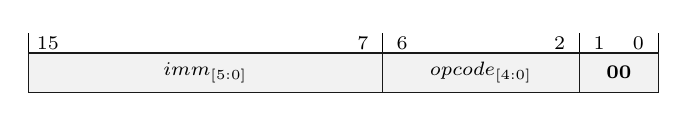
\begin{tikzpicture}[scale=0.5]
\node at (15.500000,1.250000) [font=\scriptsize] {1};
\node at (16.500000,1.250000) [font=\scriptsize] {0};
\node at (10.500000,1.250000) [font=\scriptsize] {6};
\node at (14.500000,1.250000) [font=\scriptsize] {2};
\node at (9.500000,1.250000) [font=\scriptsize] {7};
\node at (1.500000,1.250000) [font=\scriptsize] {15};
\draw (15.000000,1.000000) -- (15.000000,1.500000);
\draw (10.000000,1.000000) -- (10.000000,1.500000);
\draw (1.000000,1.000000) -- (1.000000,1.500000);
\draw (17.000000,1.000000) -- (17.000000,1.500000);
\fill [black!5]  (15.000000,0.000000) rectangle (17.000000,1.000000);
\draw [black!90]  (15.000000,0.000000) rectangle (17.000000,1.000000);
\node at (16.000000,0.500000) [font=\scriptsize] {\textbf{00}};
\fill [black!5]  (10.000000,0.000000) rectangle (15.000000,1.000000);
\draw [black!90]  (10.000000,0.000000) rectangle (15.000000,1.000000);
\node at (12.500000,0.500000) [font=\scriptsize] {$opcode_{[4:0]}$};
\fill [black!5]  (1.000000,0.000000) rectangle (10.000000,1.000000);
\draw [black!90]  (1.000000,0.000000) rectangle (10.000000,1.000000);
\node at (5.500000,0.500000) [font=\scriptsize] {$imm_{[5:0]}$};
\end{tikzpicture}
\caption{16-bit large immediate.}
\label{fig:glyph-iform-opi-16}
\end{figure}

\begin{figure}[H]
\centering
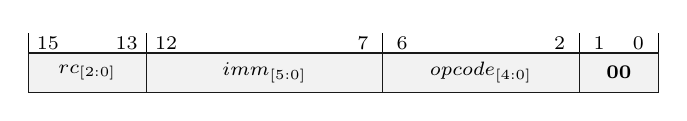
\begin{tikzpicture}[scale=0.5]
\node at (15.500000,1.250000) [font=\scriptsize] {1};
\node at (16.500000,1.250000) [font=\scriptsize] {0};
\node at (10.500000,1.250000) [font=\scriptsize] {6};
\node at (14.500000,1.250000) [font=\scriptsize] {2};
\node at (4.500000,1.250000) [font=\scriptsize] {12};
\node at (9.500000,1.250000) [font=\scriptsize] {7};
\node at (1.500000,1.250000) [font=\scriptsize] {15};
\node at (3.500000,1.250000) [font=\scriptsize] {13};
\draw (15.000000,1.000000) -- (15.000000,1.500000);
\draw (10.000000,1.000000) -- (10.000000,1.500000);
\draw (4.000000,1.000000) -- (4.000000,1.500000);
\draw (1.000000,1.000000) -- (1.000000,1.500000);
\draw (17.000000,1.000000) -- (17.000000,1.500000);
\fill [black!5]  (15.000000,0.000000) rectangle (17.000000,1.000000);
\draw [black!90]  (15.000000,0.000000) rectangle (17.000000,1.000000);
\node at (16.000000,0.500000) [font=\scriptsize] {\textbf{00}};
\fill [black!5]  (10.000000,0.000000) rectangle (15.000000,1.000000);
\draw [black!90]  (10.000000,0.000000) rectangle (15.000000,1.000000);
\node at (12.500000,0.500000) [font=\scriptsize] {$opcode_{[4:0]}$};
\fill [black!5]  (4.000000,0.000000) rectangle (10.000000,1.000000);
\draw [black!90]  (4.000000,0.000000) rectangle (10.000000,1.000000);
\node at (7.000000,0.500000) [font=\scriptsize] {$imm_{[5:0]}$};
\fill [black!5]  (1.000000,0.000000) rectangle (4.000000,1.000000);
\draw [black!90]  (1.000000,0.000000) rectangle (4.000000,1.000000);
\node at (2.500000,0.500000) [font=\scriptsize] {$rc_{[2:0]}$};
\end{tikzpicture}
\caption{16-bit one operand with immediate.}
\label{fig:glyph-iform-op1ri-16}
\end{figure}

\begin{figure}[H]
\centering
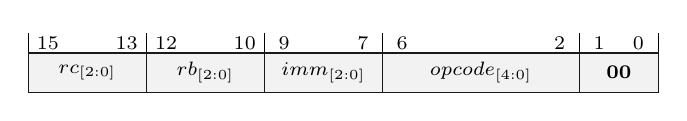
\begin{tikzpicture}[scale=0.5]
\node at (15.500000,1.250000) [font=\scriptsize] {1};
\node at (16.500000,1.250000) [font=\scriptsize] {0};
\node at (10.500000,1.250000) [font=\scriptsize] {6};
\node at (14.500000,1.250000) [font=\scriptsize] {2};
\node at (7.500000,1.250000) [font=\scriptsize] {9};
\node at (9.500000,1.250000) [font=\scriptsize] {7};
\node at (4.500000,1.250000) [font=\scriptsize] {12};
\node at (6.500000,1.250000) [font=\scriptsize] {10};
\node at (1.500000,1.250000) [font=\scriptsize] {15};
\node at (3.500000,1.250000) [font=\scriptsize] {13};
\draw (15.000000,1.000000) -- (15.000000,1.500000);
\draw (10.000000,1.000000) -- (10.000000,1.500000);
\draw (7.000000,1.000000) -- (7.000000,1.500000);
\draw (4.000000,1.000000) -- (4.000000,1.500000);
\draw (1.000000,1.000000) -- (1.000000,1.500000);
\draw (17.000000,1.000000) -- (17.000000,1.500000);
\fill [black!5]  (15.000000,0.000000) rectangle (17.000000,1.000000);
\draw [black!90]  (15.000000,0.000000) rectangle (17.000000,1.000000);
\node at (16.000000,0.500000) [font=\scriptsize] {\textbf{00}};
\fill [black!5]  (10.000000,0.000000) rectangle (15.000000,1.000000);
\draw [black!90]  (10.000000,0.000000) rectangle (15.000000,1.000000);
\node at (12.500000,0.500000) [font=\scriptsize] {$opcode_{[4:0]}$};
\fill [black!5]  (7.000000,0.000000) rectangle (10.000000,1.000000);
\draw [black!90]  (7.000000,0.000000) rectangle (10.000000,1.000000);
\node at (8.500000,0.500000) [font=\scriptsize] {$imm_{[2:0]}$};
\fill [black!5]  (4.000000,0.000000) rectangle (7.000000,1.000000);
\draw [black!90]  (4.000000,0.000000) rectangle (7.000000,1.000000);
\node at (5.500000,0.500000) [font=\scriptsize] {$rb_{[2:0]}$};
\fill [black!5]  (1.000000,0.000000) rectangle (4.000000,1.000000);
\draw [black!90]  (1.000000,0.000000) rectangle (4.000000,1.000000);
\node at (2.500000,0.500000) [font=\scriptsize] {$rc_{[2:0]}$};
\end{tikzpicture}
\caption{16-bit two operand with immediate.}
\label{fig:glyph-iform-op2ri-16}
\end{figure}

\begin{figure}[H]
\centering
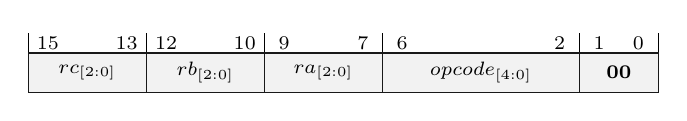
\begin{tikzpicture}[scale=0.5]
\node at (15.500000,1.250000) [font=\scriptsize] {1};
\node at (16.500000,1.250000) [font=\scriptsize] {0};
\node at (10.500000,1.250000) [font=\scriptsize] {6};
\node at (14.500000,1.250000) [font=\scriptsize] {2};
\node at (7.500000,1.250000) [font=\scriptsize] {9};
\node at (9.500000,1.250000) [font=\scriptsize] {7};
\node at (4.500000,1.250000) [font=\scriptsize] {12};
\node at (6.500000,1.250000) [font=\scriptsize] {10};
\node at (1.500000,1.250000) [font=\scriptsize] {15};
\node at (3.500000,1.250000) [font=\scriptsize] {13};
\draw (15.000000,1.000000) -- (15.000000,1.500000);
\draw (10.000000,1.000000) -- (10.000000,1.500000);
\draw (7.000000,1.000000) -- (7.000000,1.500000);
\draw (4.000000,1.000000) -- (4.000000,1.500000);
\draw (1.000000,1.000000) -- (1.000000,1.500000);
\draw (17.000000,1.000000) -- (17.000000,1.500000);
\fill [black!5]  (15.000000,0.000000) rectangle (17.000000,1.000000);
\draw [black!90]  (15.000000,0.000000) rectangle (17.000000,1.000000);
\node at (16.000000,0.500000) [font=\scriptsize] {\textbf{00}};
\fill [black!5]  (10.000000,0.000000) rectangle (15.000000,1.000000);
\draw [black!90]  (10.000000,0.000000) rectangle (15.000000,1.000000);
\node at (12.500000,0.500000) [font=\scriptsize] {$opcode_{[4:0]}$};
\fill [black!5]  (7.000000,0.000000) rectangle (10.000000,1.000000);
\draw [black!90]  (7.000000,0.000000) rectangle (10.000000,1.000000);
\node at (8.500000,0.500000) [font=\scriptsize] {$ra_{[2:0]}$};
\fill [black!5]  (4.000000,0.000000) rectangle (7.000000,1.000000);
\draw [black!90]  (4.000000,0.000000) rectangle (7.000000,1.000000);
\node at (5.500000,0.500000) [font=\scriptsize] {$rb_{[2:0]}$};
\fill [black!5]  (1.000000,0.000000) rectangle (4.000000,1.000000);
\draw [black!90]  (1.000000,0.000000) rectangle (4.000000,1.000000);
\node at (2.500000,0.500000) [font=\scriptsize] {$rc_{[2:0]}$};
\end{tikzpicture}
\caption{16-bit three operand.}
\label{fig:glyph-iform-op3r-16}
\end{figure}

\newpage
\subsubsection{32-bit instruction forms}

this section details the layout of the 32-bit instruction forms:

\begin{figure}[H]
\centering
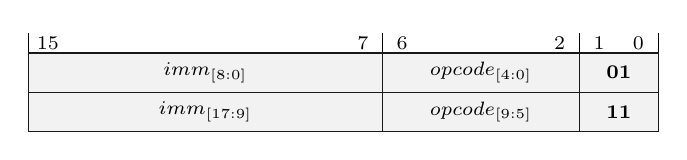
\begin{tikzpicture}[scale=0.5]
\node at (15.500000,1.250000) [font=\scriptsize] {1};
\node at (16.500000,1.250000) [font=\scriptsize] {0};
\node at (10.500000,1.250000) [font=\scriptsize] {6};
\node at (14.500000,1.250000) [font=\scriptsize] {2};
\node at (1.500000,1.250000) [font=\scriptsize] {15};
\node at (9.500000,1.250000) [font=\scriptsize] {7};
\draw (15.000000,1.000000) -- (15.000000,1.500000);
\draw (10.000000,1.000000) -- (10.000000,1.500000);
\draw (1.000000,1.000000) -- (1.000000,1.500000);
\draw (17.000000,1.000000) -- (17.000000,1.500000);
\fill [black!5]  (15.000000,0.000000) rectangle (17.000000,1.000000);
\draw [black!90]  (15.000000,0.000000) rectangle (17.000000,1.000000);
\node at (16.000000,0.500000) [font=\scriptsize] {\textbf{01}};
\fill [black!5]  (10.000000,0.000000) rectangle (15.000000,1.000000);
\draw [black!90]  (10.000000,0.000000) rectangle (15.000000,1.000000);
\node at (12.500000,0.500000) [font=\scriptsize] {$opcode_{[4:0]}$};
\fill [black!5]  (1.000000,0.000000) rectangle (10.000000,1.000000);
\draw [black!90]  (1.000000,0.000000) rectangle (10.000000,1.000000);
\node at (5.500000,0.500000) [font=\scriptsize] {$imm_{[8:0]}$};
\fill [black!5]  (15.000000,-1.000000) rectangle (17.000000,0.000000);
\draw [black!90]  (15.000000,-1.000000) rectangle (17.000000,0.000000);
\node at (16.000000,-0.500000) [font=\scriptsize] {\textbf{11}};
\fill [black!5]  (10.000000,-1.000000) rectangle (15.000000,0.000000);
\draw [black!90]  (10.000000,-1.000000) rectangle (15.000000,0.000000);
\node at (12.500000,-0.500000) [font=\scriptsize] {$opcode_{[9:5]}$};
\fill [black!5]  (1.000000,-1.000000) rectangle (10.000000,0.000000);
\draw [black!90]  (1.000000,-1.000000) rectangle (10.000000,0.000000);
\node at (5.500000,-0.500000) [font=\scriptsize] {$imm_{[17:9]}$};
\end{tikzpicture}
\caption{32-bit large immediate.}
\label{fig:glyph-iform-opi-32}
\end{figure}

\begin{figure}[H]
\centering
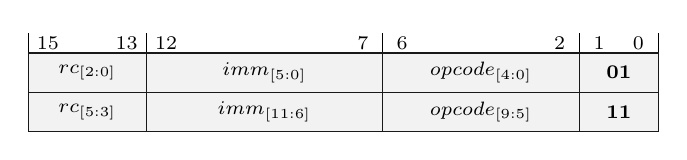
\begin{tikzpicture}[scale=0.5]
\node at (15.500000,1.250000) [font=\scriptsize] {1};
\node at (16.500000,1.250000) [font=\scriptsize] {0};
\node at (10.500000,1.250000) [font=\scriptsize] {6};
\node at (14.500000,1.250000) [font=\scriptsize] {2};
\node at (4.500000,1.250000) [font=\scriptsize] {12};
\node at (9.500000,1.250000) [font=\scriptsize] {7};
\node at (1.500000,1.250000) [font=\scriptsize] {15};
\node at (3.500000,1.250000) [font=\scriptsize] {13};
\draw (15.000000,1.000000) -- (15.000000,1.500000);
\draw (10.000000,1.000000) -- (10.000000,1.500000);
\draw (4.000000,1.000000) -- (4.000000,1.500000);
\draw (1.000000,1.000000) -- (1.000000,1.500000);
\draw (17.000000,1.000000) -- (17.000000,1.500000);
\fill [black!5]  (15.000000,0.000000) rectangle (17.000000,1.000000);
\draw [black!90]  (15.000000,0.000000) rectangle (17.000000,1.000000);
\node at (16.000000,0.500000) [font=\scriptsize] {\textbf{01}};
\fill [black!5]  (10.000000,0.000000) rectangle (15.000000,1.000000);
\draw [black!90]  (10.000000,0.000000) rectangle (15.000000,1.000000);
\node at (12.500000,0.500000) [font=\scriptsize] {$opcode_{[4:0]}$};
\fill [black!5]  (4.000000,0.000000) rectangle (10.000000,1.000000);
\draw [black!90]  (4.000000,0.000000) rectangle (10.000000,1.000000);
\node at (7.000000,0.500000) [font=\scriptsize] {$imm_{[5:0]}$};
\fill [black!5]  (1.000000,0.000000) rectangle (4.000000,1.000000);
\draw [black!90]  (1.000000,0.000000) rectangle (4.000000,1.000000);
\node at (2.500000,0.500000) [font=\scriptsize] {$rc_{[2:0]}$};
\fill [black!5]  (15.000000,-1.000000) rectangle (17.000000,0.000000);
\draw [black!90]  (15.000000,-1.000000) rectangle (17.000000,0.000000);
\node at (16.000000,-0.500000) [font=\scriptsize] {\textbf{11}};
\fill [black!5]  (10.000000,-1.000000) rectangle (15.000000,0.000000);
\draw [black!90]  (10.000000,-1.000000) rectangle (15.000000,0.000000);
\node at (12.500000,-0.500000) [font=\scriptsize] {$opcode_{[9:5]}$};
\fill [black!5]  (4.000000,-1.000000) rectangle (10.000000,0.000000);
\draw [black!90]  (4.000000,-1.000000) rectangle (10.000000,0.000000);
\node at (7.000000,-0.500000) [font=\scriptsize] {$imm_{[11:6]}$};
\fill [black!5]  (1.000000,-1.000000) rectangle (4.000000,0.000000);
\draw [black!90]  (1.000000,-1.000000) rectangle (4.000000,0.000000);
\node at (2.500000,-0.500000) [font=\scriptsize] {$rc_{[5:3]}$};
\end{tikzpicture}
\caption{32-bit one operand with immediate.}
\label{fig:glyph-iform-op1ri-32}
\end{figure}

\begin{figure}[H]
\centering
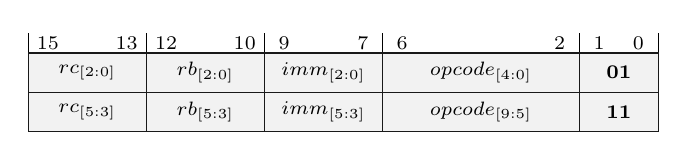
\begin{tikzpicture}[scale=0.5]
\node at (15.500000,1.250000) [font=\scriptsize] {1};
\node at (16.500000,1.250000) [font=\scriptsize] {0};
\node at (10.500000,1.250000) [font=\scriptsize] {6};
\node at (14.500000,1.250000) [font=\scriptsize] {2};
\node at (7.500000,1.250000) [font=\scriptsize] {9};
\node at (9.500000,1.250000) [font=\scriptsize] {7};
\node at (4.500000,1.250000) [font=\scriptsize] {12};
\node at (6.500000,1.250000) [font=\scriptsize] {10};
\node at (1.500000,1.250000) [font=\scriptsize] {15};
\node at (3.500000,1.250000) [font=\scriptsize] {13};
\draw (15.000000,1.000000) -- (15.000000,1.500000);
\draw (10.000000,1.000000) -- (10.000000,1.500000);
\draw (7.000000,1.000000) -- (7.000000,1.500000);
\draw (4.000000,1.000000) -- (4.000000,1.500000);
\draw (1.000000,1.000000) -- (1.000000,1.500000);
\draw (17.000000,1.000000) -- (17.000000,1.500000);
\fill [black!5]  (15.000000,0.000000) rectangle (17.000000,1.000000);
\draw [black!90]  (15.000000,0.000000) rectangle (17.000000,1.000000);
\node at (16.000000,0.500000) [font=\scriptsize] {\textbf{01}};
\fill [black!5]  (10.000000,0.000000) rectangle (15.000000,1.000000);
\draw [black!90]  (10.000000,0.000000) rectangle (15.000000,1.000000);
\node at (12.500000,0.500000) [font=\scriptsize] {$opcode_{[4:0]}$};
\fill [black!5]  (7.000000,0.000000) rectangle (10.000000,1.000000);
\draw [black!90]  (7.000000,0.000000) rectangle (10.000000,1.000000);
\node at (8.500000,0.500000) [font=\scriptsize] {$imm_{[2:0]}$};
\fill [black!5]  (4.000000,0.000000) rectangle (7.000000,1.000000);
\draw [black!90]  (4.000000,0.000000) rectangle (7.000000,1.000000);
\node at (5.500000,0.500000) [font=\scriptsize] {$rb_{[2:0]}$};
\fill [black!5]  (1.000000,0.000000) rectangle (4.000000,1.000000);
\draw [black!90]  (1.000000,0.000000) rectangle (4.000000,1.000000);
\node at (2.500000,0.500000) [font=\scriptsize] {$rc_{[2:0]}$};
\fill [black!5]  (15.000000,-1.000000) rectangle (17.000000,0.000000);
\draw [black!90]  (15.000000,-1.000000) rectangle (17.000000,0.000000);
\node at (16.000000,-0.500000) [font=\scriptsize] {\textbf{11}};
\fill [black!5]  (10.000000,-1.000000) rectangle (15.000000,0.000000);
\draw [black!90]  (10.000000,-1.000000) rectangle (15.000000,0.000000);
\node at (12.500000,-0.500000) [font=\scriptsize] {$opcode_{[9:5]}$};
\fill [black!5]  (7.000000,-1.000000) rectangle (10.000000,0.000000);
\draw [black!90]  (7.000000,-1.000000) rectangle (10.000000,0.000000);
\node at (8.500000,-0.500000) [font=\scriptsize] {$imm_{[5:3]}$};
\fill [black!5]  (4.000000,-1.000000) rectangle (7.000000,0.000000);
\draw [black!90]  (4.000000,-1.000000) rectangle (7.000000,0.000000);
\node at (5.500000,-0.500000) [font=\scriptsize] {$rb_{[5:3]}$};
\fill [black!5]  (1.000000,-1.000000) rectangle (4.000000,0.000000);
\draw [black!90]  (1.000000,-1.000000) rectangle (4.000000,0.000000);
\node at (2.500000,-0.500000) [font=\scriptsize] {$rc_{[5:3]}$};
\end{tikzpicture}
\caption{32-bit two operand with immediate.}
\label{fig:glyph-iform-op2ri-32}
\end{figure}

\begin{figure}[H]
\centering
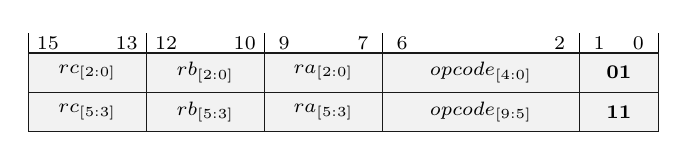
\begin{tikzpicture}[scale=0.5]
\node at (15.500000,1.250000) [font=\scriptsize] {1};
\node at (16.500000,1.250000) [font=\scriptsize] {0};
\node at (10.500000,1.250000) [font=\scriptsize] {6};
\node at (14.500000,1.250000) [font=\scriptsize] {2};
\node at (7.500000,1.250000) [font=\scriptsize] {9};
\node at (9.500000,1.250000) [font=\scriptsize] {7};
\node at (4.500000,1.250000) [font=\scriptsize] {12};
\node at (6.500000,1.250000) [font=\scriptsize] {10};
\node at (1.500000,1.250000) [font=\scriptsize] {15};
\node at (3.500000,1.250000) [font=\scriptsize] {13};
\draw (15.000000,1.000000) -- (15.000000,1.500000);
\draw (10.000000,1.000000) -- (10.000000,1.500000);
\draw (7.000000,1.000000) -- (7.000000,1.500000);
\draw (4.000000,1.000000) -- (4.000000,1.500000);
\draw (1.000000,1.000000) -- (1.000000,1.500000);
\draw (17.000000,1.000000) -- (17.000000,1.500000);
\fill [black!5]  (15.000000,0.000000) rectangle (17.000000,1.000000);
\draw [black!90]  (15.000000,0.000000) rectangle (17.000000,1.000000);
\node at (16.000000,0.500000) [font=\scriptsize] {\textbf{01}};
\fill [black!5]  (10.000000,0.000000) rectangle (15.000000,1.000000);
\draw [black!90]  (10.000000,0.000000) rectangle (15.000000,1.000000);
\node at (12.500000,0.500000) [font=\scriptsize] {$opcode_{[4:0]}$};
\fill [black!5]  (7.000000,0.000000) rectangle (10.000000,1.000000);
\draw [black!90]  (7.000000,0.000000) rectangle (10.000000,1.000000);
\node at (8.500000,0.500000) [font=\scriptsize] {$ra_{[2:0]}$};
\fill [black!5]  (4.000000,0.000000) rectangle (7.000000,1.000000);
\draw [black!90]  (4.000000,0.000000) rectangle (7.000000,1.000000);
\node at (5.500000,0.500000) [font=\scriptsize] {$rb_{[2:0]}$};
\fill [black!5]  (1.000000,0.000000) rectangle (4.000000,1.000000);
\draw [black!90]  (1.000000,0.000000) rectangle (4.000000,1.000000);
\node at (2.500000,0.500000) [font=\scriptsize] {$rc_{[2:0]}$};
\fill [black!5]  (15.000000,-1.000000) rectangle (17.000000,0.000000);
\draw [black!90]  (15.000000,-1.000000) rectangle (17.000000,0.000000);
\node at (16.000000,-0.500000) [font=\scriptsize] {\textbf{11}};
\fill [black!5]  (10.000000,-1.000000) rectangle (15.000000,0.000000);
\draw [black!90]  (10.000000,-1.000000) rectangle (15.000000,0.000000);
\node at (12.500000,-0.500000) [font=\scriptsize] {$opcode_{[9:5]}$};
\fill [black!5]  (7.000000,-1.000000) rectangle (10.000000,0.000000);
\draw [black!90]  (7.000000,-1.000000) rectangle (10.000000,0.000000);
\node at (8.500000,-0.500000) [font=\scriptsize] {$ra_{[5:3]}$};
\fill [black!5]  (4.000000,-1.000000) rectangle (7.000000,0.000000);
\draw [black!90]  (4.000000,-1.000000) rectangle (7.000000,0.000000);
\node at (5.500000,-0.500000) [font=\scriptsize] {$rb_{[5:3]}$};
\fill [black!5]  (1.000000,-1.000000) rectangle (4.000000,0.000000);
\draw [black!90]  (1.000000,-1.000000) rectangle (4.000000,0.000000);
\node at (2.500000,-0.500000) [font=\scriptsize] {$rc_{[5:3]}$};
\end{tikzpicture}
\caption{32-bit three operand.}
\label{fig:glyph-iform-op3r-32}
\end{figure}

\subsection{instruction decoding}

the instruction size encoding and field extension scheme has been designed
to minimize complexity for parallel decoding in hardware and software.
the following table shows the instruction width combinations for
various width parallel instruction decoders.
\\
\begin{table}[h]
\centering
\small
\begin{tabular}{|c|c|c|c|c|}
\hline
\textbf{Packets} & \textbf{Bits} & \textbf{Bytes} & $\bm{n_{combos}}$ & $\bm{\log_2(n)}$ \\
\hline
1-wide  & 16-bit   & 2  & 1     & \fmtlogtwo{1} \\
2-wide  & 32-bit   & 4  & 16    & \fmtlogtwo{16} \\
4-wide  & 64-bit   & 8  & 58    & \fmtlogtwo{58} \\
8-wide  & 128-bit  & 16 & 574   & \fmtlogtwo{574} \\
16-wide & 256-bit  & 32 & 51904 & \fmtlogtwo{51904} \\
\hline
\end{tabular}
\caption{instruction decode combinations}
\label{tab:instruction-decode-combos}
\end{table}

\newpage
\section{Register file}

the glyph register file is extensible due to the variable length
instruction format and supports a different number of registers
depending on the instruction size.
\begin{itemize}[itemsep=0pt]
\item 16-bit instruction packet can access 8 registers with up to 3 operands.
\item 32-bit instruction packet can access 64 registers with up to 3 operands.
\item 64-bit instruction packet can access 64 registers with up to 6 operands.
\end{itemize}

\par\noindent
the register state accessible by the 16-bit instruction packet is comprised of:
\begin{itemize}[itemsep=0pt]
\item \emph{program counter} register (aligned to 2 bytes).
\item \emph{immediate base} register (aligned to 64 bytes).
\item 8 \texttimes general purpose registers (\emph{r0} through \emph{r7}).
\item 1 \texttimes predicate register (\emph{flag}).
\end{itemize}

\par\noindent
the following diagram shows the register state accessible by the 16-bit
instruction packet:
\\

\begin{figure}[H]
\centering
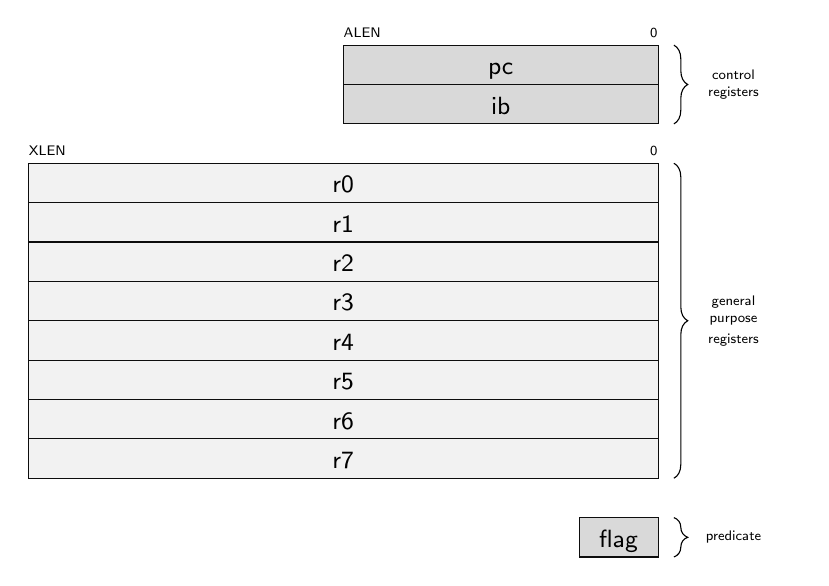
\begin{tikzpicture}[scale=0.5]
\begin{scope}[every node/.style={font=\small, inner sep=0pt, right}]
\foreach \x in {0,...,7}
  \fill [black!5] (0,\x)    rectangle (16,\x+1);
\foreach \x in {0,...,7}
  \draw [black!95] (0,\x)    rectangle (16,\x+1);
\node [font=\small,anchor=base] at (8,0.25)  {\textsf{r7}};
\node [font=\small,anchor=base] at (8,1.25)  {\textsf{r6}};
\node [font=\small,anchor=base] at (8,2.25)  {\textsf{r5}};
\node [font=\small,anchor=base] at (8,3.25)  {\textsf{r4}};
\node [font=\small,anchor=base] at (8,4.25)  {\textsf{r3}};
\node [font=\small,anchor=base] at (8,5.25)  {\textsf{r2}};
\node [font=\small,anchor=base] at (8,6.25)  {\textsf{r1}};
\node [font=\small,anchor=base] at (8,7.25)  {\textsf{r0}};

\node [font=\tiny,anchor=base west] at (8,11.2)  {\textsf{ALEN}};
\node [font=\tiny,anchor=base east] at (16,11.2)  {\textsf{0}};
\node [font=\tiny,anchor=base west] at (0,8.2)  {\textsf{XLEN}};
\node [font=\tiny,anchor=base east] at (16,8.2)  {\textsf{0}};

\fill [black!15] (8,9)    rectangle (16,10);
\draw [black!95] (8,9)    rectangle (16,10);

\fill [black!15] (8,10)    rectangle (16,11);
\draw [black!95] (8,10)    rectangle (16,11);

\fill [black!15] (14,-2)    rectangle (16,-1);
\draw [black!95] (14,-2)    rectangle (16,-1);

\node [font=\small,anchor=base] at (12,9.25)  {\textsf{ib}};
\node [font=\small,anchor=base] at (12,10.25)  {\textsf{pc}};
\node [font=\small,anchor=base] at (15,-1.75)  {\textsf{flag}};

\draw [decorate,decoration={brace,amplitude=5pt,mirror,raise=2mm}]
    (16,9) -- (16,11) node[midway,xshift=1mm,align=center,font=\tiny,
        text width=17mm,anchor=west]{\textsf{\shortstack{control\\registers}}};

\draw [decorate,decoration={brace,amplitude=5pt,mirror,raise=2mm}]
    (16,0) -- (16,8) node[midway,xshift=1mm,align=center,font=\tiny,
        text width=17mm,anchor=west]{\textsf{\shortstack{general\\purpose\\registers}}};

\draw [decorate,decoration={brace,amplitude=5pt,mirror,raise=2mm}]
    (16,-2) -- (16,-1) node[midway,xshift=1mm,align=center,font=\tiny,
        text width=17mm,anchor=west]{\textsf{\shortstack{predicate}}};

\end{scope}
\end{tikzpicture}
\caption{register state accessible by 16-bit instruction packet.}
\label{fig:glyph-register-state-64}
\end{figure}

\par\noindent
the use of
\emph{ALEN}\footnote{\emph{ALEN} refers to the width of addresses in bits.} and
\emph{XLEN}\footnote{\emph{XLEN} refers to the width of general purpose registers in bits.}
parameters is to indicate that the width of addresses can be less than
the width of the general purpose registers.

\newpage
\section{Example pipeline}

an illustrative micro-architecture is proposed based on the classic 5-stage
RISC micro-architecture~\cite{patterson-hennessy} with the addition of an
\emph{operand fetch} stage and a \emph{constant memory} port. this revised
6-stage micro-architecture is composed of the following pipeline stages:

\begin{itemize}[itemsep=0pt]
\item \textsf{IF} --- \emph{instruction fetch}: reads instructions from memory
into a fetch buffer.
\item \textsf{ID} --- \emph{instruction decode}: decodes instruction length, opcode,
and operands.
\item \textsf{OF} --- \emph{operand fetch}: reads operands from register file
and constant memory.
\item \textsf{EX} --- \emph{execute}: performs logical operations or
arithmetic on the operands.
\item \textsf{MA} --- \emph{memory access}: loads data from or stores data to memory.
\item \textsf{WB} --- \emph{writeback}: writes results back to the register file.
\end{itemize}

\par\noindent
a simplified micro-architecture using those pipeline stages might look like this:
this example omits hazard detection and forwarding logic for the sake of simplicity.
\\
\begin{figure}[H]
\centering
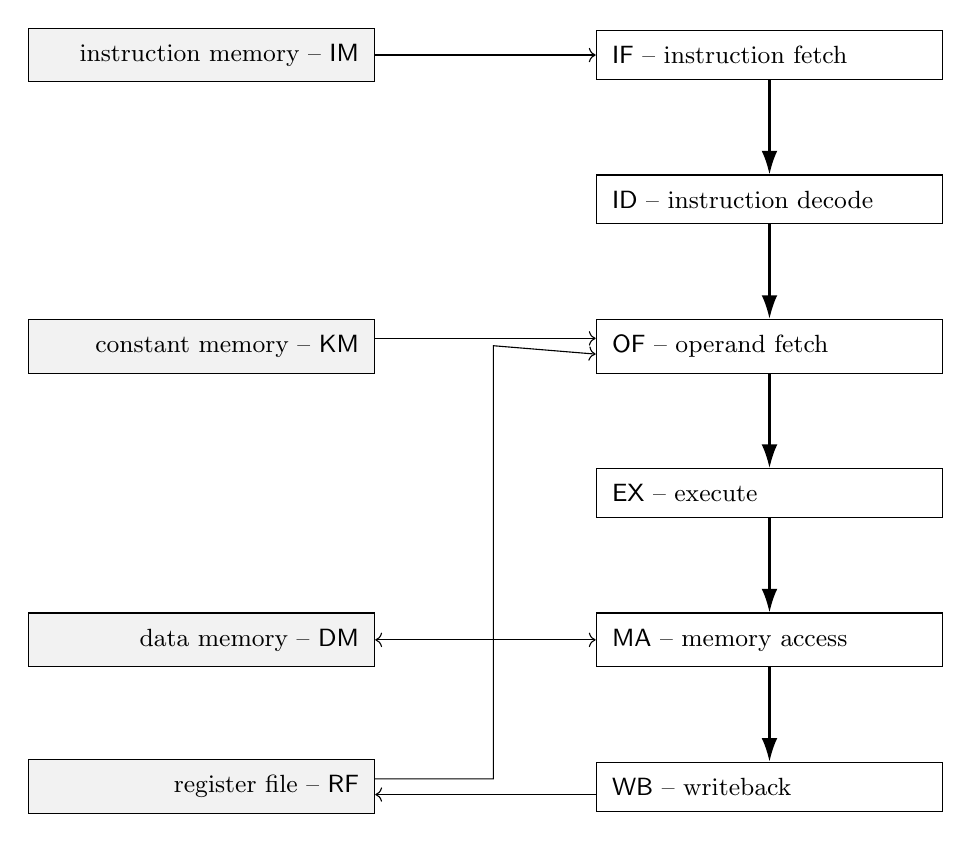
\begin{tikzpicture}[
  every node/.style={font=\small},
  stage/.style={rectangle, draw=black, thick, align=center},
  sidebox/.style={rectangle, draw=black, thick, fill=gray!10},
  arrow/.style={-{Latex[length=3mm, width=2mm]}, thick},
  node distance=12mm
]

% Pipeline stages
\tikzstyle{stage} = [draw, align=left, text width=40mm, minimum height=5mm, inner sep=2mm]
\tikzstyle{sidebox} = [draw, fill=black!5, align=right, text width=40mm, minimum height=5mm, inner sep=2mm]

\node[stage] (IF) {\textsf{IF} -- instruction fetch};
\node[stage, below=of IF] (ID) {\textsf{ID} -- instruction decode};
\node[stage, below=of ID] (OF) {\textsf{OF} -- operand fetch};
\node[stage, below=of OF] (EX) {\textsf{EX} -- execute};
\node[stage, below=of EX] (MA) {\textsf{MA} -- memory access};
\node[stage, below=of MA] (WB) {\textsf{WB} -- writeback};

% Arrows between pipeline stages
\draw[arrow] (IF) -- (ID);
\draw[arrow] (ID) -- (OF);
\draw[arrow] (OF) -- (EX);
\draw[arrow] (EX) -- (MA);
\draw[arrow] (MA) -- (WB);

% Side components
\node[sidebox, left=2.8cm of IF] (instrmem) {instruction memory -- \textsf{IM}};
\draw[->] (instrmem.east) -- (IF.west);

\node[sidebox, left=2.8cm of OF] (constmem) {constant memory -- \textsf{KM}};
\draw[->] ([yshift=1mm]constmem.east) -- ([yshift=1mm]OF.west);

\node[sidebox, left=2.8cm of MA] (datamem) {data memory -- \textsf{DM}};
\draw[<->] (datamem.east) -- (MA.west);

\node[sidebox, left=2.8cm of WB] (regfile) {register file -- \textsf{RF}};
\draw[->] ([yshift=1mm]regfile.east) -- ++(1.5,0) -- ++(0,5.5) -- ([yshift=-1mm]OF.west);
\draw[<-] ([yshift=-1mm]regfile.east) -- ([yshift=-1mm]WB.west);

\end{tikzpicture}
\caption{sample 6-stage micro-architecture with support for constant memory.}
\label{fig:glyph-6-stage-uarch}
\end{figure}

\chapter{System}

\section{System registers}
the architecture provides several control and status registers for
floating-point control and status, time, trap handling, address translation,
timers, inter-thread interrupts, and debug.

\begin{table}[h]
\centering
\footnotesize
\begin{tabular}{|l|l|l|}
\hline
\textbf{no.} & \textbf{name} & \textbf{description} \\
\hline
\multicolumn{3}{|l|}{\textbf{user-level registers}} \\ \hline
\texttt{0x00} & fpcontrol & floating-point control \\
\texttt{0x01} & fpstatus  & floating-point status \\
\texttt{0x02} & ctime     & clock time \\
\texttt{0x03} & cfreq     & clock frequency \\
\hline
\multicolumn{3}{|l|}{\textbf{privileged trap registers}} \\ \hline
\texttt{0x10} & tcontrol  & trap control \\
\texttt{0x11} & tstatus   & trap status \\
\texttt{0x12} & tscratch  & trap scratch \\
\texttt{0x13} & tepc      & trap exception program counter  \\
\texttt{0x14} & teib      & trap exception immediate base \\
\texttt{0x15} & tval      & trap value \\
\texttt{0x16} & tcause    & trap cause \\
\texttt{0x17} & tack      & trap acknowledge \\
\texttt{0x18} & thpc      & trap handler program counter  \\
\texttt{0x19} & thib      & trap handler immediate base \\
\hline
\multicolumn{3}{|l|}{\textbf{privileged system registers}} \\ \hline
\texttt{0x20} & scontrol  & system control \\
\texttt{0x21} & sstatus   & system status \\
\texttt{0x22} & sptr      & system page table root \\
\texttt{0x23} & saddr     & system thread address \\
\texttt{0x24} & starget   & system target address \\
\texttt{0x25} & smessage  & system message interrupt \\
\texttt{0x26} & stimer    & system deadline timer \\
\texttt{0x27} & sie       & system interrupt enable \\
\texttt{0x28} & sip       & system interrupt pending \\
\hline
\multicolumn{3}{|l|}{\textbf{privileged debug registers}} \\ \hline
\texttt{0x31} & dstatus    & debug status \\
\texttt{0x32} & dcycle     & debug cycle counter \\
\texttt{0x33} & dinst      & debug instruction counter \\
\texttt{0x34} & dstop      & debug stop instruction \\
\texttt{0x35} & dfetch     & monitored fetch address \\
\texttt{0x36} & dread      & monitored read address \\
\texttt{0x37} & dwrite     & monitored write address \\
\hline
\end{tabular}
\caption{system registers}
\label{tab:system-registers}
\end{table}

\newpage
\subsection{user-level registers}
the section describes the user-level registers.

\subsubsection{floating-point control (\texttt{fpcontrol})}
\texttt{fpcontrol} contains control information for floating-point
operations. the \texttt{RM} field is a read-write and contains
the current floating-point rounding mode.
\\
\begin{tikzpicture}[scale=0.45]
\draw [black!95] (0,0)    rectangle (32,1);
\draw [black!95] (30,0)    rectangle (32,1);
\node [font=\tiny,anchor=base] at (31.5,1.25)  {\textsf{0}};
\node [font=\tiny,anchor=base] at (30.5,1.25)  {\textsf{1}};
\node [font=\small,anchor=base] at (31,0.25)  {\texttt{RM}};
\end{tikzpicture}

\begin{table}[h]
\centering
\footnotesize
\begin{tabular}{|l|l|l|}
\hline
\textbf{no.} & \textbf{name} & \textbf{description} \\
\hline
\verb|0| & RN   & round to nearest (even) \\
\verb|1| & RD   & round down (towards $-\infty$) \\
\verb|2| & RU   & round up (towards $+\infty$) \\
\verb|3| & RZ   & round towards zero (truncate) \\
\hline
\end{tabular}
\caption{floating-point control round mode field}
\label{tab:floating-point-control-round-mode-field}
\end{table}

\subsubsection{floating-point status (\texttt{fpstatus})}
\texttt{fpstatus} contains status information for floating-point
operations. the \texttt{I, Z, U, O,} and \texttt{P} fields are
read-write and contain accrued floating-point exceptions.
\\
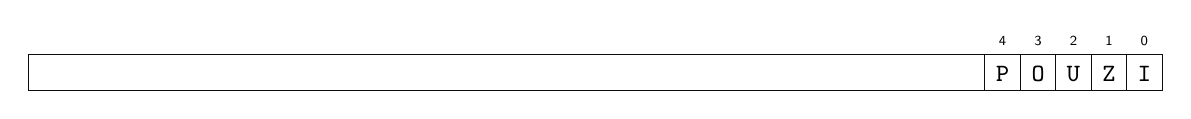
\begin{tikzpicture}[scale=0.45]
\draw [black!95] (0,0)    rectangle (32,1);
\draw [black!95] (31,0)    rectangle (32,1);
\node [font=\tiny,anchor=base] at (31.5,1.25)  {\textsf{0}};
\node [font=\small,anchor=base] at (31.5,0.25)  {\texttt{I}};
\draw [black!95] (30,0)    rectangle (31,1);
\node [font=\tiny,anchor=base] at (30.5,1.25)  {\textsf{1}};
\node [font=\small,anchor=base] at (30.5,0.25)  {\texttt{Z}};
\draw [black!95] (29,0)    rectangle (30,1);
\node [font=\tiny,anchor=base] at (29.5,1.25)  {\textsf{2}};
\node [font=\small,anchor=base] at (29.5,0.25)  {\texttt{U}};
\draw [black!95] (28,0)    rectangle (29,1);
\node [font=\tiny,anchor=base] at (28.5,1.25)  {\textsf{3}};
\node [font=\small,anchor=base] at (28.5,0.25)  {\texttt{O}};
\draw [black!95] (27,0)    rectangle (28,1);
\node [font=\tiny,anchor=base] at (27.5,1.25)  {\textsf{4}};
\node [font=\small,anchor=base] at (27.5,0.25)  {\texttt{P}};
\end{tikzpicture}

\begin{table}[h]
\centering
\footnotesize
\begin{tabular}{|l|l|l|}
\hline
\textbf{no.} & \textbf{name} & \textbf{description} \\
\hline
\verb|1 << 0| & I   & invalid operation \\
\verb|1 << 1| & Z   & divide by zero \\
\verb|1 << 2| & U   & numeric underflow \\
\verb|1 << 3| & O   & numeric overflow \\
\verb|1 << 4| & P   & inexact result \\
\hline
\end{tabular}
\caption{floating-point status flags}
\label{tab:floating-point-status-flags}
\end{table}

\subsubsection{clock time (\texttt{ctime})}
\texttt{ctime} is a read-only register containing the wall-clock
tick counter since power on in clock tick units denoted by \texttt{cfreq}.

\subsubsection{clock frequency (\texttt{cfreq})}
\texttt{cfreq} is a read-only register containing the wall-clock
tick interval in picoseconds; \(\frac{10^{12}}{f} \) where \( f \)
is the frequency in Hertz (Hz).

\newpage
\subsection{privileged trap registers}
the section describes the privileged trap registers.

\subsubsection{trap control (\texttt{tcontrol})}
\texttt{tcontrol} is a read-write register containing control bits. the
\texttt{I} field is read-write and controls whether system interrupts
are enabled for this hardware thread.
\\
\begin{tikzpicture}[scale=0.45]
\draw [black!95] (0,0)    rectangle (32,1);
\draw [black!95] (31,0)    rectangle (32,1);
\node [font=\tiny,anchor=base] at (31.5,1.25)  {\textsf{0}};
\node [font=\small,anchor=base] at (31.5,0.25)  {\texttt{I}};
\end{tikzpicture}

\begin{table}[h]
\centering
\footnotesize
\begin{tabular}{|l|l|l|}
\hline
\textbf{no.} & \textbf{name} & \textbf{description} \\
\hline
\verb|1 << 0| & I   & system interrupt enable \\
\hline
\end{tabular}
\caption{trap control fields}
\label{tab:trap-control-fields}
\end{table}

\subsubsection{trap status (\texttt{tstatus})}
\texttt{tstatus} contains status bits for the current trap. the \texttt{T}
field is read-only and indicates whether a timer interrupt is pending.
the \texttt{V} field is read-only and indicates whether a virtual
interrupt is pending.
\\
\begin{tikzpicture}[scale=0.45]
\draw [black!95] (0,0)    rectangle (32,1);
\draw [black!95] (31,0)    rectangle (32,1);
\node [font=\tiny,anchor=base] at (31.5,1.25)  {\textsf{0}};
\node [font=\small,anchor=base] at (31.5,0.25)  {\texttt{T}};
\draw [black!95] (30,0)    rectangle (31,1);
\node [font=\tiny,anchor=base] at (30.5,1.25)  {\textsf{1}};
\node [font=\small,anchor=base] at (30.5,0.25)  {\texttt{V}};
\end{tikzpicture}

\begin{table}[h]
\centering
\footnotesize
\begin{tabular}{|l|l|l|}
\hline
\textbf{no.} & \textbf{name} & \textbf{description} \\
\hline
\verb|1 << 0| & T   & timer interrupt pending \\
\verb|1 << 1| & V   & virtual interrupt pending \\
\hline
\end{tabular}
\caption{trap status fields}
\label{tab:trap-status-fields}
\end{table}

\subsubsection{trap scratch (\texttt{tscratch})}
\texttt{tscratch} is a read-write save register for use during trap handling.

\subsubsection{trap exception program counter (\texttt{tepc})}
\texttt{tepc} is a read-only register which contains the \emph{program
counter} address before the trap.

\subsubsection{trap exception immedidate base (\texttt{teib})}
\texttt{teib} is a read-only register which contains the \emph{immediate
base} address before the trap.

\newpage
\subsubsection{trap value (\texttt{tval})}
\texttt{tval} is a read-only register with a word indicating the identity
of the trap, and may contain:

\begin{itemize}[itemsep=0pt]
\item the faulting instruction word for \emph{break} and \emph{illegal instruction exceptions}.
\item the faulting address for \emph{access} and \emph{page faults}.
\item the message value for \emph{virtual interrupts}.
\item the system clock time for \emph{timer interrupts}.
\end{itemize}

\subsubsection{trap cause (\texttt{tcause})}
\texttt{tcause} is a read-only register that contains the cause of the
current trap, and may contain:

\begin{table}[h]
\centering
\footnotesize
\begin{tabular}{|l|l|l|}
\hline
\textbf{no.} & \textbf{name} & \textbf{description} \\
\hline
\multicolumn{3}{|l|}{\textbf{system exceptions}} \\ \hline
\verb|1| & break-instruction   & break instruction exception \\
\verb|2| & illegal-instruction & illegal instruction exception \\
\verb|3| & debug-monitor       & debug monitor exception \\
\verb|4| & misaligned-fetch    & fetch misaligned \\
\verb|5| & misaligned-load     & load misaligned \\
\verb|6| & misaligned-store    & store misaligned \\
\verb|7| & access-fault-fetch  & fetch access fault \\
\verb|8| & access-fault-load   & load access fault \\
\verb|9| & access-fault-store  & store access fault \\
\verb|10| & page-fault-fetch   & fetch page fault \\
\verb|11| & page-fault-load    & load page fault \\
\verb|12| & page-fault-store   & store page fault \\
\hline
\multicolumn{3}{|l|}{\textbf{system interrupts}} \\ \hline
\verb|30| & timer-interrupt     & timer interrupt \\
\verb|31| & virtual-interrupt   & virtual interrupt \\
\hline
\verb|32| & interrupt-0         & interrupt pin 0 \\
\ldots & \ldots & \ldots \\
\verb|63| & interrupt-31        & interrupt pin 31 \\
\hline
\end{tabular}
\caption{trap causes}
\label{tab:trap-causes}
\end{table}

\subsubsection{trap acknowledge (\texttt{tack})}
\texttt{tack} is a write-only register where the trap cause is written
to acknowledge the trap so that interrupts are not delivered
while state is being saved, and for double-faults to be detected.

\subsubsection{trap handler program counter (\texttt{thpc})}
\texttt{thpc} is a read-write register containing the address of the
system trap handler routine.

\subsubsection{trap handler immediate base (\texttt{thib})}
\texttt{thib} is a read-write register containing the address of the
system trap handler constants.

\newpage
\subsection{privileged system registers}
the section describes the privileged system registers.

\subsubsection{system control (\texttt{scontrol})}
\texttt{scontrol} is a read-write register containing system control
information. the \texttt{A} field controls whether the user pages can
be read or written by the supervisor. the \texttt{E} field controls
whether user pages can be executed by the supervisor.
\\
\begin{tikzpicture}[scale=0.45]
\draw [black!95] (0,0)    rectangle (32,1);
\draw [black!95] (31,0)    rectangle (32,1);
\node [font=\tiny,anchor=base] at (31.5,1.25)  {\textsf{0}};
\node [font=\small,anchor=base] at (31.5,0.25)  {\texttt{A}};
\draw [black!95] (30,0)    rectangle (31,1);
\node [font=\tiny,anchor=base] at (30.5,1.25)  {\textsf{1}};
\node [font=\small,anchor=base] at (30.5,0.25)  {\texttt{E}};
\end{tikzpicture}

\begin{table}[h]
\centering
\footnotesize
\begin{tabular}{|l|l|l|}
\hline
\textbf{no.} & \textbf{name} & \textbf{description} \\
\hline
\verb|1 << 0| & A   & supervisor access user pages \\
\verb|1 << 1| & E   & supervisor execute user pages \\
\hline
\end{tabular}
\caption{system control fields}
\label{tab:system-control-fields}
\end{table}

\subsubsection{system status (\texttt{sstatus})}
\texttt{sstatus} is a read-only register containing system status.
the \texttt{U} field indicates the processor is operating in user-mode.
this register cannot be read in user-mode so it will return zero.
\\
\begin{tikzpicture}[scale=0.45]
\draw [black!95] (0,0)    rectangle (32,1);
\draw [black!95] (31,0)    rectangle (32,1);
\node [font=\tiny,anchor=base] at (31.5,1.25)  {\textsf{0}};
\node [font=\small,anchor=base] at (31.5,0.25)  {\texttt{U}};
\end{tikzpicture}

\begin{table}[h]
\centering
\footnotesize
\begin{tabular}{|l|l|l|}
\hline
\textbf{no.} & \textbf{name} & \textbf{description} \\
\hline
\verb|1 << 0| & U   & user mode \\
\hline
\end{tabular}
\caption{system status fields}
\label{tab:system-status-fields}
\end{table}

\subsubsection{system page table root (\texttt{sptr})}
\texttt{sptr} is a read-write register containing the page table root
for address translation on this hardware thread. the \emph{ASID} field
contains the address space identifier for the current thread. the
\emph{PPN} field contains the physical page number of the page table
root structure.
\\
\par\noindent
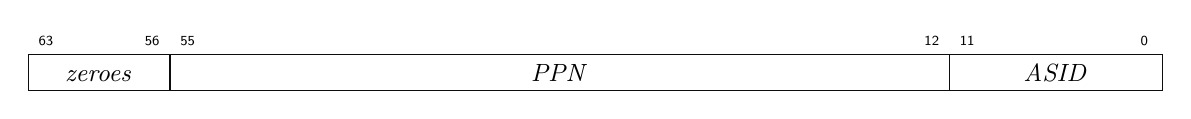
\begin{tikzpicture}[scale=0.45]
\draw [black!95] (0,0)    rectangle (32,1);
\draw [black!95] (26,0)    rectangle (32,1);
\node [font=\tiny,anchor=base] at (31.5,1.25)  {\textsf{0}};
\node [font=\tiny,anchor=base] at (26.5,1.25)  {\textsf{11}};
\node [font=\small,anchor=base] at (29,0.25)  {\emph{ASID}};
\draw [black!95] (4,0)    rectangle (26,1);
\node [font=\tiny,anchor=base] at (25.5,1.25)  {\textsf{12}};
\node [font=\tiny,anchor=base] at (4.5,1.25)  {\textsf{55}};
\node [font=\small,anchor=base] at (15,0.25)  {\emph{PPN}};
\draw [black!95] (0.0,0)   rectangle (4,1);
\node [font=\tiny,anchor=base] at (0.5,1.25)  {\textsf{63}};
\node [font=\tiny,anchor=base] at (3.5,1.25)  {\textsf{56}};
\node [font=\small,anchor=base] at (2.0,0.25)  {\emph{zeroes}};
\end{tikzpicture}

\newpage
\subsubsection{system address (\texttt{saddr})}
\texttt{saddr} is a read-only register containing the unique system-wide
address for this hardware thread. the system-wide address is used as the
target for inter-thread virtual interrupts.

\subsubsection{system target (\texttt{starget})}
\texttt{starget} is a read-write register containing the system-wide
address for a hardware thread that is the target of an edge-triggered
virtual interrupt. there are two special addresses:

\begin{itemize}[itemsep=0pt]
\item a target address of all-zeros is the boot service processor.
\item a target address of all-ones is the broadcast address for all threads.
\end{itemize}

\subsubsection{system message (\texttt{smessage})}
\texttt{smessage} is a write-only register that causes an edge-triggered
virtual interrupt to be queued to the hardware thread set in \texttt{starget}.
virtual interrupts are marked pending in the \texttt{V} field of the
\texttt{tstatus} register.
if interrupts are not enabled on the target hardware thread, the virtual
interrupt is delivered when interrupts are next enabled.

\subsubsection{system timer (\texttt{stimer})}
\texttt{stimer} is a read-write register containing the deadline timer
for this hardware thread. when the system clock reaches the value in the
register, a \emph{timer interrupt} is triggered.
timer interrupts are marked pending in the \texttt{T} field of the
\texttt{tstatus} register.
if interrupts are not enabled on this hardware thread, the timer interrupt
is delivered when interrupts are next enabled.

\subsubsection{system interrupt enable (\texttt{sie})}
\texttt{sie} is a read-write register that contains interrupt enable flags
for 32 wired interrupt pins.

\subsubsection{system interrupt pending (\texttt{sip})}
\texttt{sip} is a read-only register that contains interrupt pending flags
for 32 wired interrupt pins.

\newpage
\subsection{privileged debug registers}
the section describes the privileged debug registers.

\subsubsection{debug status (\texttt{dstatus})}
\texttt{dstatus} is a read-only register containing status bits for debug
monitor execeptions.
\\
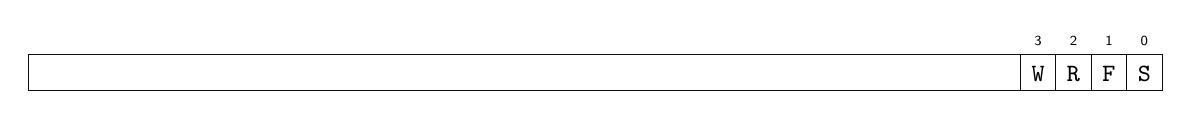
\begin{tikzpicture}[scale=0.45]
\draw [black!95] (0,0)    rectangle (32,1);
\draw [black!95] (31,0)    rectangle (32,1);
\node [font=\tiny,anchor=base] at (31.5,1.25)  {\textsf{0}};
\node [font=\small,anchor=base] at (31.5,0.25)  {\texttt{S}};
\draw [black!95] (30,0)    rectangle (31,1);
\node [font=\tiny,anchor=base] at (30.5,1.25)  {\textsf{1}};
\node [font=\small,anchor=base] at (30.5,0.25)  {\texttt{F}};
\draw [black!95] (29,0)    rectangle (30,1);
\node [font=\tiny,anchor=base] at (29.5,1.25)  {\textsf{2}};
\node [font=\small,anchor=base] at (29.5,0.25)  {\texttt{R}};
\draw [black!95] (28,0)    rectangle (29,1);
\node [font=\tiny,anchor=base] at (28.5,1.25)  {\textsf{3}};
\node [font=\small,anchor=base] at (28.5,0.25)  {\texttt{W}};
\end{tikzpicture}

\begin{table}[h]
\centering
\footnotesize
\begin{tabular}{|l|l|l|}
\hline
\textbf{no.} & \textbf{name} & \textbf{description} \\
\hline
\verb|1 << 0| & S   & stopping instruction \\
\verb|1 << 1| & F   & fetch monitor address \\
\verb|1 << 2| & R   & load monitor address \\
\verb|1 << 3| & W   & store monitor address \\
\hline
\end{tabular}
\caption{debug status fields}
\label{tab:debug-status-fields}
\end{table}

\subsubsection{debug cycle counter (\texttt{dcycle})}
\texttt{dcycle} is a read-only register containing the number of cycles
retired since power on.

\subsubsection{debug instruction counter (\texttt{dinst})}
\texttt{dinst} is a read-only register containing the number of instructions
retired since power on.

\subsubsection{debug stop instruction (\texttt{dstop})}
\texttt{dstop} is a read-write register containing an instruction number
to halt execution on and raise a \emph{debug monitor exception}.

\subsubsection{debug monitor fetch (\texttt{dfetch})}
\texttt{dfetch} is a read-write register containing a memory fetch address
to monitor for and halt execution on and raise a \emph{debug monitor
exception} for a matching memory fetch address.

\subsubsection{debug monitor read (\texttt{dread})}
\texttt{dread} is a read-write register containing the memory load
address to monitor for and halt execution on and raise a \emph{debug
monitor exception} for a matching memory load address.

\subsubsection{debug monitor write (\texttt{dwrite})}
\texttt{dwrite} is a read-write register containing the memory store
address to monitor for and halt execution on and raise a \emph{debug
monitor exception} for a matching memory store address.

\newpage
\section{Address translation}

the architecture provides for page-based virtual to physical address
translation using a page table \emph{trie structure} composed of index
pages containing arrays of page table entries. a page walker reads the
structure from the root pointer to leaf entries to translate virtual
addresses into physical addresses.

\subsection{page table structure}
the section describes the page table structure and dimensions for memory
address translation pointed to by the \emph{system page table root} register.
\\
\begin{table}[h]
\centering
\footnotesize
\begin{tabular}{|l|l|l|l|l|l|l|l|}
\hline
\textbf{Levels} & \textbf{PN\tablefootnote{Page Number} bits} &
\textbf{PO\tablefootnote{Page Offset} bits} &
\textbf{Virt bits} & \textbf{Phys bits} & \textbf{Entry bits} &
\textbf{Entries} & \textbf{Page sizes} \\
\hline
4 & 9 & 12 & 48 & 56 & 64 & 512 & 4KiB, 2Mib, 1GiB \\
\hline
\end{tabular}
\caption{64-bit page table dimensions}
\label{tab:64-bit-page-table-dimensions}
\end{table}

\par\noindent
page table entry structures are grouped together into arrays stored
within index pages, where each entry in the index maps to a
page number extracted from the virtual address.
\\
\begin{figure}[H]
\centering
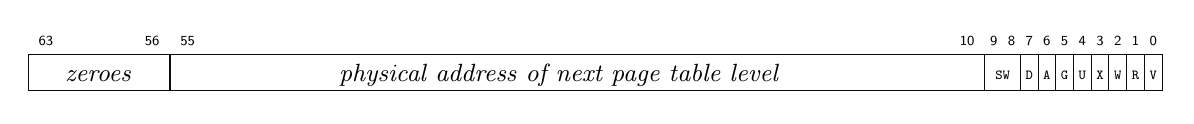
\begin{tikzpicture}[scale=0.45]
\draw [black!95] (0,0)    rectangle (32,1);
\draw [black!95] (31.5,0)    rectangle (32,1);
\node [font=\tiny,anchor=base] at (31.75,1.25)  {\textsf{0}};
\node [font=\tiny,anchor=base] at (31.75,0.3)  {\texttt{V}};
\draw [black!95] (31.0,0)    rectangle (31.5,1);
\node [font=\tiny,anchor=base] at (31.25,1.25)  {\textsf{1}};
\node [font=\tiny,anchor=base] at (31.25,0.3)  {\texttt{R}};
\draw [black!95] (30.5,0)    rectangle (31.0,1);
\node [font=\tiny,anchor=base] at (30.75,1.25)  {\textsf{2}};
\node [font=\tiny,anchor=base] at (30.75,0.3)  {\texttt{W}};
\draw [black!95] (30.0,0)    rectangle (30.5,1);
\node [font=\tiny,anchor=base] at (30.25,1.25)  {\textsf{3}};
\node [font=\tiny,anchor=base] at (30.25,0.3)  {\texttt{X}};
\draw [black!95] (29.5,0)    rectangle (30.0,1);
\node [font=\tiny,anchor=base] at (29.75,1.25)  {\textsf{4}};
\node [font=\tiny,anchor=base] at (29.75,0.3)  {\texttt{U}};
\draw [black!95] (29.0,0)    rectangle (29.5,1);
\node [font=\tiny,anchor=base] at (29.25,1.25)  {\textsf{5}};
\node [font=\tiny,anchor=base] at (29.25,0.3)  {\texttt{G}};
\draw [black!95] (28.5,0)    rectangle (29.0,1);
\node [font=\tiny,anchor=base] at (28.75,1.25)  {\textsf{6}};
\node [font=\tiny,anchor=base] at (28.75,0.3)  {\texttt{A}};
\draw [black!95] (28.0,0)    rectangle (28.5,1);
\node [font=\tiny,anchor=base] at (28.25,1.25)  {\textsf{7}};
\node [font=\tiny,anchor=base] at (28.25,0.3)  {\texttt{D}};
\draw [black!95] (27.0,0)    rectangle (28.0,1);
\node [font=\tiny,anchor=base] at (27.75,1.25)  {\textsf{8}};
\node [font=\tiny,anchor=base] at (27.25,1.25)  {\textsf{9}};
\node [font=\tiny,anchor=base] at (27.5,0.3)  {\texttt{SW}};
\draw [black!95] (4,0)    rectangle (27.0,1);
\node [font=\tiny,anchor=base] at (26.5,1.25)  {\textsf{10}};
\node [font=\tiny,anchor=base] at (4.5,1.25)  {\textsf{55}};
\node [font=\small,anchor=base] at (15,0.25)  {\emph{physical address of next page table level}};
\draw [black!95] (0.0,0)   rectangle (4,1);
\node [font=\tiny,anchor=base] at (0.5,1.25)  {\textsf{63}};
\node [font=\tiny,anchor=base] at (3.5,1.25)  {\textsf{56}};
\node [font=\small,anchor=base] at (2.0,0.25)  {\emph{zeroes}};
\end{tikzpicture}
\caption{64-bit page table entry structure.}
\label{fig:64-bit-pte-structure}
\end{figure}

\par\noindent
page table entry bits indicate the type and permission of a page in
the \emph{trie-based} page table. entries with the \emph{read, write}
and \emph{exec} bits clear are \emph{internal nodes}, referred to as
\emph{pointer nodes} within the context \emph{trie-based} page tables.
\\
\begin{table}[h]
\centering
\footnotesize
\begin{tabular}{|l|l|l|}
\hline
\textbf{no.} & \textbf{name} & \textbf{description} \\
\hline
\verb|1 << 0| & V   & valid \\
\verb|1 << 1| & R   & read \\
\verb|1 << 2| & W   & write \\
\verb|1 << 3| & X   & execute \\
\verb|1 << 4| & U   & user \\
\verb|1 << 5| & G   & global \\
\verb|1 << 6| & A   & accessed \\
\verb|1 << 7| & D   & dirty \\
\verb|3 << 8| & SW   & software \\
\hline
\end{tabular}
\caption{64-bit page table entry fields}
\label{tab:64-bit-page-table-entry-fields}
\end{table}

\newpage
\subsection{page table walker}
the page table walker performs page table lookups to translate virtual
addresses into physical addresses. the page table walker reads the page
table root pointer then walks the \emph{trie-based} page table structure
to find a leaf entry containing a physical page address.

\begin{figure}[H]
\centering
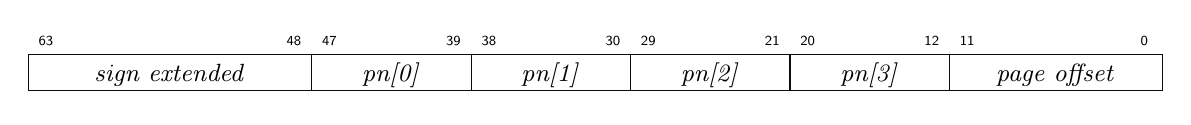
\begin{tikzpicture}[scale=0.45]
\draw [black!95] (0,0)    rectangle (32,1);
\draw [black!95] (26,0)   rectangle (32,1);
\node [font=\tiny,anchor=base] at (26.5,1.25)  {\textsf{11}};
\node [font=\tiny,anchor=base] at (31.5,1.25)  {\textsf{0}};
\node [font=\small,anchor=base] at (29,0.25)  {\emph{page offset}};
\draw [black!95] (21.5,0)   rectangle (26,1);
\node [font=\tiny,anchor=base] at (22.0,1.25)  {\textsf{20}};
\node [font=\tiny,anchor=base] at (25.5,1.25)  {\textsf{12}};
\node [font=\small,anchor=base] at (23.75,0.25)  {\emph{pn[3]}};
\draw [black!95] (17.0,0)   rectangle (21.5,1);
\node [font=\tiny,anchor=base] at (17.5,1.25)  {\textsf{29}};
\node [font=\tiny,anchor=base] at (21.0,1.25)  {\textsf{21}};
\node [font=\small,anchor=base] at (19.25,0.25)  {\emph{pn[2]}};
\draw [black!95] (12.5,0)   rectangle (17.0,1);
\node [font=\tiny,anchor=base] at (13.0,1.25)  {\textsf{38}};
\node [font=\tiny,anchor=base] at (16.5,1.25)  {\textsf{30}};
\node [font=\small,anchor=base] at (14.75,0.25)  {\emph{pn[1]}};
\draw [black!95] (8.0,0)   rectangle (12.5,1);
\node [font=\tiny,anchor=base] at (8.5,1.25)  {\textsf{47}};
\node [font=\tiny,anchor=base] at (12.0,1.25)  {\textsf{39}};
\node [font=\small,anchor=base] at (10.25,0.25)  {\emph{pn[0]}};
\draw [black!95] (0.0,0)   rectangle (8.0,1);
\node [font=\tiny,anchor=base] at (0.5,1.25)  {\textsf{63}};
\node [font=\tiny,anchor=base] at (7.5,1.25)  {\textsf{48}};
\node [font=\small,anchor=base] at (4.0,0.25)  {\emph{sign extended}};
\end{tikzpicture}
\caption{64-bit lookup virtual address structure.}
\label{fig:64-bit-lookup-virtual-address-structure}
\end{figure}

\begin{figure}[H]
\centering
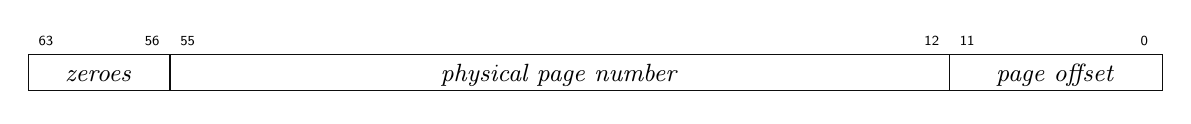
\begin{tikzpicture}[scale=0.45]
\draw [black!95] (0,0)    rectangle (32,1);
\draw [black!95] (26,0)   rectangle (32,1);
\node [font=\tiny,anchor=base] at (26.5,1.25)  {\textsf{11}};
\node [font=\tiny,anchor=base] at (31.5,1.25)  {\textsf{0}};
\node [font=\small,anchor=base] at (29,0.25)  {\emph{page offset}};
\draw [black!95] (4.0,0)   rectangle (26,1);
\node [font=\tiny,anchor=base] at (4.5,1.25)  {\textsf{55}};
\node [font=\tiny,anchor=base] at (25.5,1.25)  {\textsf{12}};
\node [font=\small,anchor=base] at (15.0,0.25)  {\emph{physical page number}};
\draw [black!95] (0.0,0)   rectangle (4,1);
\node [font=\tiny,anchor=base] at (0.5,1.25)  {\textsf{63}};
\node [font=\tiny,anchor=base] at (3.5,1.25)  {\textsf{56}};
\node [font=\small,anchor=base] at (2.0,0.25)  {\emph{zeroes}};
\end{tikzpicture}
\caption{64-bit translated physical address structure.}
\label{fig:64-bit-translated-physical-address-structure}
\end{figure}

\par\noindent
the page table address translation process and rules are as follows:

\begin{algorithm}
\caption{translate virtual address to physical address}
\small
\begin{algorithmic}[1]

 \Function{translate}{$op,va$}
  \If {$\lnot\Call{check\_canonical}{\mathit{va}, \mathit{va\_bits}}$}
    \Comment{check address is sign-extended}
    \State \textbf{raise} \textbf{fault}
  \EndIf
  \State $\mathit{ppn} \gets \mathit{sptr.ppn}$
  \Comment{fetch the page table root pointer}
  \For{$\mathit{level} \gets 1$ to $\mathit{num\_levels}$}
      \State $\mathit{shift} \gets (\mathit{num\_levels} - \mathit{level}) \times
        \mathit{pn\_bits} + \mathit{po\_bits}$
      \Comment{calculate virtual page number}
      \State $\mathit{vpn} \gets (\mathit{va} >> \mathit{shift}) \land
        ((1 << \mathit{pn\_bits}) - 1)$
      \State $\mathit{pte} \gets \Call{load}{(\mathit{ppn}
        << \mathit{po\_bits}) + \mathit{vpn} \times \mathit{pte\_size}}$
      \If {$(\lnot\mathit{pte.V}) \lor (\mathit{pte.W} \land \lnot\mathit{pte.R})$}
        \Comment{check valid and write must have read}
        \State \textbf{raise} \textbf{fault}
      \ElsIf {$\lnot(\mathit{pte.R} \lor \mathit{pte.W} \lor \mathit{pte.X})$}
      \Comment{no read, write or exec is a pointer}
        \State $\mathit{ppn} \gets \mathit{pte.ppn}$
        \State \textbf{continue}
      \ElsIf{$(\mathit{op.R} \land \lnot\mathit{pte.R}) \lor (\mathit{op.W} \land
        \lnot\mathit{pte.W}) \lor (\mathit{op.X} \land \lnot\mathit{pte.X})$}
        \Comment{check access perms}
        \State \textbf{raise} \textbf{fault}
      \ElsIf {$(\mathit{op.R} \land \lnot\mathit{pte.A}) \lor
          (\mathit{op.W} \land \lnot\mathit{pte.D})$}
        \Comment{check accessed or dirty}
        \State \textbf{raise} \textbf{fault}
      \ElsIf {$\lnot\mathit{sstatus.U} \land \lnot\mathit{scontrol.E} \land
          \mathit{pte.U} \land \mathit{op.X}$}
        \Comment{check execute user page}
        \State \textbf{raise} \textbf{fault}
      \ElsIf {$\lnot\mathit{sstatus.U} \land \lnot\mathit{scontrol.A} \land
          \mathit{pte.U} \land (\mathit{op.R} \lor \mathit{op.W})$}
        \Comment{check access user page}
        \State \textbf{raise} \textbf{fault}
      \ElsIf {$\mathit{pte.ppn} \land ((1 << (\mathit{shift} -
          \mathit{po\_bits})) - 1) \ne 0$}
        \Comment{check superpage is aligned}
        \State \textbf{raise} \textbf{fault}
      \EndIf
      \State \Return $(\mathit{ppn} << \mathit{po\_bits}) + (\mathit{va} \land
      ((1 << (\mathit{level} \times \mathit{pn\_bits} + \mathit{po\_bits})) - 1))$
  \EndFor
 \EndFunction

\end{algorithmic}
\end{algorithm}

\chapter{Instructions} \label{sec:instructions}

\section{Instruction listing --- 16-bit}

\needspace{8\baselineskip}
\subsection{break}
\insnimmnine{uimm}{00000}{00}{\textbf{break}\: uimm9}
\\
the \emph{break} instruction causes a debugger trap.
\emph{program counter} and trap cause are saved to privileged
registers for the operating system to dispatch to a debugger
and the \emph{program counter} is set to a trap vector address.

\needspace{8\baselineskip}
\subsection{j}
\insnimmnine{simm}{00001}{00}{\textbf{j}\: simm9 \times 2}
\\
the \emph{j} or \emph{jump} instruction is an unconditional branch instruction
that adds a relative immediate address to the \emph{program counter}. the
resulting \emph{program counter} address is \emph{$[pc + simm9 \times 2]$}.
\begin{Verbatim}
    pc = pc + simm9 * 2
\end{Verbatim}

\needspace{8\baselineskip}
\subsection{b}
\insnimmnine{simm}{00010}{00}{\textbf{b}\: simm9 \times 2}
\\
the \emph{b} or \emph{branch} instruction is a conditional branch instruction
that adds a relative immediate address to the \emph{program counter}. if the
\emph{flag} register has been set by a compare instruction, the resulting
\emph{program counter} address is \emph{$[pc + simm9 \times 2]$},
otherwise the \emph{program counter} is advanced normally.
\begin{Verbatim}
    if flag:
        pc = pc + simm9 * 2
\end{Verbatim}

\needspace{8\baselineskip}
\subsection{ibj}
\insnimmnine{simm}{00011}{00}{\textbf{ibj}\: simm9 \times 64}
\\
the \emph{ibj} or \emph{immediate-block-jump} instruction adds a
64-bit relative address to the \emph{immediate base} register.
the resulting \emph{immediate base} address is \emph{$[ib + simm9 \times 64]$}.
\begin{Verbatim}
    ib = ib + simm9 * 64
\end{Verbatim}

\needspace{8\baselineskip}
\subsection{link}
\insrcimmsix{fun}{uimm}{00100}{00}{\textbf{link.i64}\: fun3, ib64(uimm6)}
\\
the \emph{link} instruction loads a 64-bit constant addressed by \emph{$[ib
+ uimm6 \times 8]$} containing a \emph{i32x2} relative address vector,
which it adds it to \emph{(pc,ib)}, conditionally subtracts the source
link register \emph{(r6 or r7)}, then conditionally adds the difference
to the destination link register \emph{(r6 or r7)}, depending on the
value of \emph{fun3}. the type of linkage in \emph{fun3} can be one of:
\\
\begin{table}[h]
\centering
\footnotesize
\begin{tabular}{|l|l|l|l|l|l|}
\hline
\textbf{value} & \textbf{mnemonic} & \textbf{description} &
\textbf{link-type} & \textbf{dst-link} & \textbf{src-link} \\
\hline
0     & jib      & jump               & jump & -  & -  \\
1     & -        & -                  & -    & -  & -  \\
2     & jalib    & jump-and-link      & call & r6 & -  \\
3     & jalib    & jump-and-link      & call & r7 & -  \\
4     & jtlib    & jump-to-link       & ret  & -  & r6 \\
5     & jtlib    & jump-to-link       & ret  & -  & r7 \\
6     & jalaib   & jump-and-link-add  & tail & r6 & -  \\
7     & jalaib   & jump-and-link-add  & tail & r7 & -  \\
\hline
\end{tabular}
\caption{Link instruction functions}
\label{tab:link-instruction-functions}
\end{table}

\begin{Verbatim}
    lr = 0b110 + (fun3 & 1)
    cval = const-mem<i32x2>[ib + uimm6 * 8]
    dval = fun3 == jalaib ? cval + auth-decrypt(reg<i32x2>[lr]) : cval
    lval = fun3 == jtlib  ?        auth-decrypt(reg<i32x2>[lr]) : 0
    (dpc,dib) = dval
    (lpc,lib) = lval
    pc = pc + dpc - lpc
    ib = ib + dib - lib
    if fun3 == jalib or fun3 == jalaib:
        reg[lr] = auth-encrypt(reg<i32x2>(dpc,dib))
\end{Verbatim}

\par\noindent
the \emph{auth-encrypt} and \emph{auth-decrypt} functions are placeholders
for authenticated encryption, and decryption of relative address vectors.
authentication failures should generate a trap for the operating system to
dispatch to a control flow integrity trap handler.

\needspace{8\baselineskip}
\subsection{movh}
\insrcimmsix{rc}{uimm}{00101}{00}{\textbf{movh.i64}\: rc, ib32(uimm6)}
\\
the \emph{movh} or \emph{move-half-immediate-block} instruction loads a
32-bit constant addressed by \emph{$[ib + uimm6 \times 4]$}, which it
sign-extends to 64-bits, then saves to the \emph{rc} register.
\begin{Verbatim}
    reg[rc] = const-mem<i32>[ib + uimm6 * 4]
\end{Verbatim}

\needspace{8\baselineskip}
\subsection{movw}
\insrcimmsix{rc}{uimm}{00110}{00}{\textbf{movw.i64}\: rc, ib64(uimm6)}
\\
the \emph{movw} or \emph{move-word-immediate-block} instruction loads a
64-bit constant addressed by \emph{$[ib + uimm6 \times 8]$} then saves
it to the \emph{rc} register.
\begin{Verbatim}
    reg[rc] = const-mem<i64>[ib + uimm6 * 8]
\end{Verbatim}

\needspace{8\baselineskip}
\subsection{movi}
\insrcimmsix{rc}{simm}{00111}{00}{\textbf{movi.i64}\: rc, simm6}
\\
the \emph{movi} or \emph{move-immediate} instruction sign-extends the
immediate value in \emph{simm6} then saves the result in the \emph{rc}
register.
\begin{Verbatim}
    reg[rc] = simm6
\end{Verbatim}

\needspace{8\baselineskip}
\subsection{addi}
\insrcimmsix{rc}{simm}{01000}{00}{\textbf{addi.i64}\: rc, simm6}
\\
the \emph{addi} or \emph{add-immediate} instruction sign-extends the
immediate value in \emph{simm6} then adds it to the \emph{rc} register.
\begin{Verbatim}
    reg[rc] = reg[rc] + simm6
\end{Verbatim}

\needspace{8\baselineskip}
\subsection{srli}
\insrcimmsix{rc}{uimm}{01001}{00}{\textbf{srli.i64}\: rc, uimm6}
\\
the \emph{srli} or \emph{shift-right-logical-immediate} instruction
performs a logical right shift by \emph{uimm6} bits of the value in
the \emph{rc} register. zeros are copied into the left most bits.
\begin{Verbatim}
    reg[rc] = reg<u64>[rc] >> uimm6
\end{Verbatim}

\needspace{8\baselineskip}
\subsection{srai}
\insrcimmsix{rc}{uimm}{01010}{00}{\textbf{srai.i64}\: rc, uimm6}
\\
the \emph{srai} or \emph{shift-right-arithmetic-immediate} instruction
performs an arithmetic right shift by \emph{uimm6} bits of the value in
the \emph{rc} register. the sign is copied into the left most bits.
\begin{Verbatim}
    reg[rc] = reg<i64>[rc] >> uimm6
\end{Verbatim}

\needspace{8\baselineskip}
\subsection{slli}
\insrcimmsix{rc}{uimm}{01011}{00}{\textbf{slli.i64}\: rc, uimm6}
\\
the \emph{slli} or \emph{shift-left-logical-immediate} instruction
performs a logical left shift by \emph{uimm6} bits of the value in
the \emph{rc} register. zeros are copied into the right most bits.
\begin{Verbatim}
    reg[rc] = reg[rc] << uimm6
\end{Verbatim}

\needspace{8\baselineskip}
\subsection{addh}
\insrcimmsix{rc}{uimm}{01100}{00}{\textbf{addh.i64}\: rc, ib32(uimm6)}
\\
the \emph{addh} or \emph{add-half-immediate-block} instruction loads
a 32-bit constant addressed by \emph{$[ib + uimm6 \times 4]$}, which it
sign-extends to 64-bits, then adds to the \emph{rc} register.
\begin{Verbatim}
    reg[rc] = reg[rc] + const-mem<i32>[ib + uimm6 * 4]
\end{Verbatim}

\needspace{8\baselineskip}
\subsection{leapc}
\insrcimmsix{rc}{uimm}{01101}{00}{\textbf{leapc.i64}\: rc, ib32(uimm6)(pc)}
\\
the \emph{leapc} or \emph{load-effective-address-pc} instruction
loads a 32-bit constant addressed by \emph{$[ib + uimm6 \times 4]$},
which it sign-extends to 64-bits, adds it to the \emph{program counter},
and saves the result in the \emph{rc} register.
\begin{Verbatim}
    reg[rc] = pc + const-mem<i32>[ib + uimm6 * 4]
\end{Verbatim}

\needspace{8\baselineskip}
\subsection{loadpc}
\insrcimmsix{rc}{uimm}{01110}{00}{\textbf{loadpc.i64}\: rc, ib32(uimm6)(pc)}
\\
the \emph{loadpc} instruction loads a 32-bit constant addressed by
\emph{$[ib + uimm6 \times 4]$} which it sign-extends to 64-bit, adds it to
the \emph{program counter} to form an address, then loads a 64-bit value
from memory at that address and saves the result in the \emph{rc} register.
\begin{Verbatim}
    reg[rc] = mem<i64>[pc + const-mem<i32>[ib + uimm6 * 4]]
\end{Verbatim}

\needspace{8\baselineskip}
\subsection{storepc}
\insrcimmsix{rc}{uimm}{01111}{00}{\textbf{storepc.i64}\: rc, ib32(uimm6)(pc)}
\\
the \emph{storepc} instruction loads a 32-bit constant addressed by
\emph{$[ib + uimm6 \times 4]$} which it sign-extends to 64-bit, adds it to the
\emph{program counter} to form an address, then stores to memory at that
address a 64-bit value from the \emph{rc} register.
\begin{Verbatim}
    mem<i64>[pc + const-mem<i32>[ib + uimm6 * 4]] = reg[rc]
\end{Verbatim}

\needspace{8\baselineskip}
\subsection{load}
\insrcrbimmthree{rc}{rb}{uimm}{10000}{00}{\textbf{load.i64}\: rc, (uimm3 \times 8)(rb)}
\\
the \emph{load} instruction computes the address \emph{$[rb + uimm3 \times 8]$}
then loads a 64-bit value from memory at that address and saves the result in
the \emph{rc} register.
\begin{Verbatim}
    reg[rc] = mem<i64>[reg[rb] + uimm3 * 8]
\end{Verbatim}

\needspace{8\baselineskip}
\subsection{store}
\insrcrbimmthree{rc}{rb}{uimm}{10001}{00}{\textbf{store.i64}\: rc, (uimm3 \times 8)(rb)}
\\
the \emph{store} instruction computes the address \emph{$[rb + uimm3 \times 8]$}
then stores a 64-bit value to memory at that address containing a 64-bit value
from the \emph{rc} register.
\begin{Verbatim}
    mem<i64>[reg[rb] + uimm3 * 8] = reg[rc]
\end{Verbatim}

\needspace{8\baselineskip}
\subsection{compare}
\insrcrbimmthree{rc}{rb}{fun}{10010}{00}{\textbf{cmp.i64}\: rc, rb, fun3}
\\
the \emph{compare} instruction performs a comparison between the value in
\emph{rb} and \emph{rc} then saves the result in the \emph{flag} register.
the \emph{compare} opcode is also used to perform conditional move whereby
the \emph{rb} register is copied into the \emph{rc} if the \emph{flag}
register is set. the type of comparsion in \emph{fun3} can be one of:
\\
\begin{table}[h]
\centering
\footnotesize
\begin{tabular}{|l|l|l|}
\hline
\textbf{value} & \textbf{mnemonic}& \textbf{description} \\
\hline
0     & \emph{lt}    & \emph{less than (signed)}          \\
1     & \emph{ge}    & \emph{greather or equal (signed)}  \\
2     & \emph{eq}    & \emph{equal}                       \\
3     & \emph{ne}    & \emph{not equal}                   \\
4     & \emph{ltu}   & \emph{less than (unsigned)}        \\
5     & \emph{geu}   & \emph{greater or equal (unsigned)} \\
6     & \emph{cmov}  & \emph{conditional move}            \\
7     & \emph{ncmov} & \emph{negated conditional move}    \\
\hline
\end{tabular}
\caption{Compare instruction functions}
\label{tab:compare-instruction-functions}
\end{table}

\begin{Verbatim}
    match fun3
    | lt    -> flag = reg<i64>[rc] <  reg<i64>[rb]
    | ge    -> flag = reg<i64>[rc] >= reg<i64>[rb]
    | eq    -> flag =      reg[rc] =       reg[rb]
    | ne    -> flag =      reg[rc] !=      reg[rb]
    | ltu   -> flag = reg<u64>[rc] <  reg<u64>[rb]
    | geu   -> flag = reg<u64>[rc] >= reg<u64>[rb]
    | cmov  -> if flag:
                   reg[rc] = reg[rb]
    | ncmov -> if not flag:
                   reg[rc] = reg[rb]
\end{Verbatim}

\needspace{8\baselineskip}
\subsection{logic}
\insrcrbimmthree{rc}{rb}{fun}{10011}{00}{\textbf{logic.i64}\: rc, rb, fun3}
\\
the \emph{logic} instruction performs a logic operation on the value
in the \emph{rb} register then stores the result in the \emph{rc}
register. the type of logic operations in \emph{fun3} can be one of:
\\
\begin{table}[h]
\centering
\footnotesize
\begin{tabular}{|l|l|l|}
\hline
\textbf{value} & \textbf{mnemonic}& \textbf{description} \\
\hline
0     & \emph{mv}    & \emph{move}                 \\
1     & \emph{not}   & \emph{logical not}          \\
2     & \emph{neg}   & \emph{negate}               \\
3     & \emph{bswap} & \emph{bswap}                \\
4     & \emph{ctz}   & \emph{count trailing zeros} \\
5     & \emph{clz}   & \emph{count leading zeros}  \\
6     & \emph{ctpop} & \emph{count population}     \\
7     & \emph{sext}  & \emph{sign extend}          \\
\hline
\end{tabular}
\caption{Logic instruction functions}
\label{tab:logic-instruction-functions}
\end{table}

\begin{Verbatim}
    match fun3
    | mov   -> reg[rc] = reg[rb]
    | not   -> reg[rc] = ~reg[rb]
    | neg   -> reg[rc] = -reg[rb]
    | bswap -> reg[rc] = bswap(reg[rb])
    | ctz   -> reg[rc] = ctz(reg[rb])
    | clz   -> reg[rc] = clz(reg[rb])
    | ctpop -> reg[rc] = ctpop(reg[rb])
    | sext  -> reg[rc] = sext(reg[rb])
\end{Verbatim}

\needspace{8\baselineskip}
\subsection{pin}
\insrcrbrc{rc}{rb}{ra}{10100}{00}{\textbf{pin.i64}\: rc, rb, ra}
\\
the \emph{pin} or \emph{pack-indirect} instruction packs two absolute
addresses as an \emph{i32x2} \emph{(pc,ib)} relative address vector.
the register \emph{ra} is subtracted from the \emph{program counter},
and the register \emph{rb} is subtracted from the \emph{immediate base}
register, and the results are packed into an \emph{i32x2} relative address
vector and saved to the register \emph{rc}.
\begin{Verbatim}
    lpc   = int<i32>(pc - reg[ra])
    lib   = int<i32>(ib - reg[rb])
    lval  = (lpc,lib)
    reg[rc] = auth-encrypt(lval)
\end{Verbatim}

\needspace{8\baselineskip}
\subsection{and}
\insrcrbrc{rc}{rb}{ra}{10101}{00}{\textbf{and.i64}\: rc, rb, ra}
\\
the \emph{and} instruction performs a \emph{logical-and} of the register
\emph{rb} and the register \emph{ra} and saves the result in the
register \emph{rc}.
\begin{Verbatim}
    reg[rc] = reg[rb] & reg[ra]
\end{Verbatim}

\needspace{8\baselineskip}
\subsection{or}
\insrcrbrc{rc}{rb}{ra}{10110}{00}{\textbf{or.i64}\: rc, rb, ra}
\\
the \emph{or} instruction performs a \emph{logical-or} of the register
\emph{rb} and the register \emph{ra} and saves the result in the
register \emph{rc}.
\begin{Verbatim}
    reg[rc] = reg[rb] | reg[ra]
\end{Verbatim}

\needspace{8\baselineskip}
\subsection{xor}
\insrcrbrc{rc}{rb}{ra}{10111}{00}{\textbf{xor.i64}\: rc, rb, ra}
\\
the \emph{xor} instruction performs a \emph{logical-exclusive-or}
of the register \emph{rb} and the register \emph{ra} and saves the
result in the register \emph{rc}.
\begin{Verbatim}
    reg[rc] = reg[rb] ^ reg[ra]
\end{Verbatim}

\needspace{8\baselineskip}
\subsection{add}
\insrcrbrc{rc}{rb}{ra}{11000}{00}{\textbf{add.i64}\: rc, rb, ra}
\\
the \emph{add} instruction adds the \emph{rb} register to
the \emph{ra} register and saves the result in the \emph{rc} register.
\begin{Verbatim}
    reg[rc] = reg[rb] + reg[ra]
\end{Verbatim}

\needspace{8\baselineskip}
\subsection{srl}
\insrcrbrc{rc}{rb}{ra}{11001}{00}{\textbf{srl.i64}\: rc, rb, ra}
\\
the \emph{srl} or \emph{shift-right-logical} instruction performs a
logical right shift of the value in the \emph{rb} register by the
number of bits in register \emph{ra} then saves the result in the
\emph{rc} register.
zeros are copied into the right most bits.
\begin{Verbatim}
    reg[rc] = reg<u64>[rb] >> reg[ra]
\end{Verbatim}

\needspace{8\baselineskip}
\subsection{sra}
\insrcrbrc{rc}{rb}{ra}{11010}{00}{\textbf{sra.i64}\: rc, rb, ra}
\\
the \emph{sra} or \emph{shift-right-arithmetic} instruction performs an
arithmetic right shift of the value in the \emph{rb} register by the
number of bits in register \emph{ra} then saves the result in the
\emph{rc} register. sign is copied into the right most bits.
\begin{Verbatim}
    reg[rc] = reg<i64>[rb] >> reg[ra]
\end{Verbatim}

\needspace{8\baselineskip}
\subsection{sll}
\insrcrbrc{rc}{rb}{ra}{11011}{00}{\textbf{sll.i64}\: rc, rb, ra}
\\
the \emph{sll} or \emph{shift-left-logical} instruction performs a
logical left shift of the value in the \emph{rb} register by the
number of bits in register \emph{ra} then saves the result in the
\emph{rc} register.
\begin{Verbatim}
    reg[rc] = reg[rb] << reg[ra]
\end{Verbatim}

\needspace{8\baselineskip}
\subsection{sub}
\insrcrbrc{rc}{rb}{ra}{11100}{00}{\textbf{sub.i64}\: rc, rb, ra}
\\
the \emph{sub} instruction subtracts the \emph{ra} register from
the \emph{rb} register and saves the result in the \emph{rc} register.
\begin{Verbatim}
    reg[rc] = reg[rb] - reg[ra]
\end{Verbatim}

\needspace{8\baselineskip}
\subsection{mul}
\insrcrbrc{rc}{rb}{ra}{11101}{00}{\textbf{mul.i64}\: rc, rb, ra}
\\
the \emph{mul} instruction performs signed multiplication of the
\emph{rb} register with the \emph{ra} register and saves the
result in the \emph{rc} register.
\begin{Verbatim}
    reg[rc] = reg[rb] * reg[ra]
\end{Verbatim}

\needspace{8\baselineskip}
\subsection{div}
\insrcrbrc{rc}{rb}{ra}{11110}{00}{\textbf{div.i64}\: rc, rb, ra}
\\
the \emph{div} instruction performs signed division of the
\emph{rb} register by the \emph{ra} register and saves the
result in the \emph{rc} register. division by zero causes
the flag to be set and zero to be stored in the \emph{rc} register.
a subsequent branch can handle the division by zero.
\begin{Verbatim}
    flag = reg[ra] == 0
    if flag:
        reg[rc] = 0
    else:
        reg[rc] = reg[rb] / reg[ra]
\end{Verbatim}

\needspace{8\baselineskip}
\subsection{illegal}
\insnimmnine{uimm}{11111}{00}{\textbf{illegal}\: uimm9}
\\
the \emph{illegal} instruction causes an illegal instruction trap.
\emph{program counter} and trap cause are saved to privileged registers
for the operating system to dispatch to an illegal instruction handler
and the \emph{program counter} is set to a trap vector address.


\chapter{Assembly}

\section{Introduction}

this glyph assembly language reference begins with an introduction to
assembler and linker concepts and terminology, followed by sections
describing the glyph assembler directives, and pseudo-instruction aliases.
section~\ref{sec:instructions} contains a complete listing of instruction.

\section{Concepts}
this section covers assembler high level concepts required to understand
the concepts involved in assembling and linking executable code from
source files. the terminology used in this section is applicable to the
PE/COFF, ELF and Mach-O file formats.

\subsection{assembly}
assembly files contains assembly language directives, macros and
instructions describing program code and data. they can be handwritten
or emitted by a compiler. an assembly file is the input file to the
assembler and the output from the assembler is an object file.

\subsection{object}
object files contain compiled relocatable object code and data emitted
by the assembler. an object file cannot be run, rather it is used as
input to the linker in a program linking step which combines them to
produce an executable file or shared library.

\subsection{archive}
archive files contain collections of relocatable object files and are
typically referred to as static libraries. archive files use a simple
format that appends together a set of object files with an index listing
the object files contained in the archive. thin archive files just
contain the index listing the object files without any associated data.

\subsection{executable}
executable files contain compiled relocatable object code and data
that has been linked together by a linker in a program linking step
using multple object files, archive files and shared libraries as input.
executable files can be statically or dynamically linked. dynamically
linked executables files express dependencies on shared libraries.

\subsection{shared library}
shared library files contain compiled relocatable object code and data
that have been linked together by a linker in a program linking step
using multple object files, archive files and shared libraries as input.
shared libraries
are dynamically linked by a runtime linker, and they express dependencies
on other shared libraries which need to be loaded at runtime.

\subsection{section}
a section is a name for a region of code or data in an object file,
executable file or shared library file. the files can be made up of
multiple sections where each section corresponds to several types of
executable code or data. this list contains the most common types:

\begin{itemize}[itemsep=0pt]
\item \texttt{.text} is a read-only section containing executable code
\item \texttt{.const} is a read-only section containing immediate blocks
\item \texttt{.data} is a read-write section containing global or static variables
\item \texttt{.rodata} is a read-only section containing read-only variables
\item \texttt{.bss} is a read-write section containing uninitialized data
\end{itemize}

\subsection{segment}
segments are loadable regions of code or data in an an executable or shared
library. segments describe virtual addresses, file offsets and memory access
permissions for mapped sections. in ELF, a segment can map to one or more
sections. in PE/COFF sections are mapped directly. in Mach-O, sections are
contained within a small set of specific segment types.

\subsection{symbol}
symbols are metadata table entries that contains a name with a
mapping to an address. symbols are present in object files and dynamic
symbols are present in shared libraries and executables. they can be
referred to in relocation entries and debugging metadata.

\subsection{relocation}
relocations are metadata table entries used to update relocatable addresses
during linking. relocations contains a type, a file offset pointing to text
or data, and a pointer to a symbol name whose address needs to be updated
during the linking step. relocations can be present in object files and
dynamic relocations are present in shared libraries and executables.

\subsection{program linking}
program linking is the process of combining multiple relocatable object
files by merging and aligning sections, resolving symbol references across
files, assigning final symbol addresses, applying relocation fixups using
relocation entries, and adding debug metadata.

\newpage
\section{Directives}
the assembler implements a number of directives that control the assembly
of instructions into object files. these directives are based on the
AT\&T System V assembler~\cite{att-svr4-asm} and the GNU assembler%
~\cite{gnu-as-manual}, with some additions. they provide the ability to
include arbitrary data, align data, export symbols, switch sections,
define constants, and emit metadata.
\\
\par\noindent
the following table lists glyph assembler directives:

\begin{table}[h]
\centering
\footnotesize
\begin{tabular}{|l|l|l|}
\hline
\textbf{Directive} & \textbf{Arguments} & \textbf{Description} \\
\hline
\multicolumn{3}{|l|}{\textbf{Data directives}} \\ \hline
\texttt{.byte}   & \emph{expression-list}    & 8-bit comma separated words   \\
\texttt{.short}  & \emph{expression-list}    & 16-bit comma separated words  \\
\texttt{.long}   & \emph{expression-list}    & 32-bit comma separated words  \\
\texttt{.quad}   & \emph{expression-list}    & 64-bit comma separated words  \\
\texttt{.octa}   & \emph{expression-list}    & 128-bit comma separated words \\
\texttt{.string} & \emph{“string”}           & emit string                   \\
\texttt{.zero}   & \emph{integer}            & emit zeroes                   \\
\hline
\multicolumn{3}{|l|}{\textbf{Alignment directives}} \\ \hline
\texttt{.align}  & \emph{pow2 [,pad\_val=0] [,max]} & align to power of 2    \\
\texttt{.balign} & \emph{bytes [,pad\_val=0]}       & byte align             \\
\hline
\multicolumn{3}{|l|}{\textbf{Symbol directives}} \\ \hline
\texttt{.globl}  & \emph{symbol\_name,const\_name}  & emit symbol \emph{(global scope)}  \\
\texttt{.local}  & \emph{symbol\_name,const\_name}  & emit symbol \emph{(local scope)}   \\
\hline
\multicolumn{3}{|l|}{\textbf{Section directives}} \\ \hline
\texttt{.text}    &         & emit \texttt{.text} section or make current    \\
\texttt{.const}   &         & emit \texttt{.const} section or make current   \\
\texttt{.data}    &         & emit \texttt{.data} section or make current    \\
\texttt{.rodata}  &         & emit \texttt{.rodata} section or make current  \\
\texttt{.bss}     &         & emit \texttt{.bss} section or make current     \\
\texttt{.common}  & \emph{symbol\_name,size,align} & emit common object to
\texttt{.bss} section \\
\texttt{.section} & \emph{section\_name}    & emit section (default
\texttt{.text}) or make current \\
\hline
\multicolumn{3}{|l|}{\textbf{Miscellaneous directives}} \\ \hline
\texttt{.equ}    & \emph{name, value}       & constant definition            \\
\texttt{.file}   & \emph{“filename”}        & emit filename symbol           \\
\texttt{.ident}  & \emph{“string”}          & emit identification string     \\
\texttt{.size}   & \emph{symbol,symbol}     & emit symbol size               \\
\texttt{.type}   & \emph{symbol,@function}  & emit symbol type               \\
\hline
\end{tabular}
\caption{Assembler directives}
\label{tab:assembler-directives}
\end{table}

\newpage
\section{Pseudo-instructions}

the assembler implements a number of convenience psuedo-instruction aliases
that are formed from regular instructions, but have implicit or deduced arguments.
\\
\par\noindent
the following table lists glyph assembler pseudo instruction aliases:

\begin{table}[h]
\centering
\footnotesize
\begin{tabular}{|l|l|l|}
\hline
\textbf{Pseudo-instruction} & \textbf{Expansion} & \textbf{Description}   \\
\texttt{nop}   & \texttt{or.i64 r0,r0,r0} & no-operation                     \\
\texttt{li} \emph{rc, expression} & (several expansions) & load immediate  \\
\texttt{la} \emph{rc, symbol}     & (several expansions) & load address    \\
\texttt{call} \emph{symbol}     & \texttt{jalib.i64} \emph{ibcall(text-label,const-label)} & procedure call \\
\texttt{ret}                    & \texttt{jtlib.i64} \emph{ibret(text-label,const-label)} & procedure return \\
\texttt{jib.i64} \emph{ib64(uimm6)} & \texttt{link.i64} \emph{ib64(uimm6),} \texttt{jib}
 & jump-immmediate-block \\
\texttt{jalib.i64} \emph{rc, ib64(uimm6)} & \texttt{link.i64} \emph{rc, ib64(uimm6),} \texttt{jalib}
 & jump-and-link-immmediate-block \\
\texttt{jtlib.i64} \emph{rc, ib64(uimm6)} & \texttt{link.i64} \emph{rc, ib64(uimm6),} \texttt{jtlib}
 & jump-to-link-immmediate-block \\
\texttt{jalaib.i64} \emph{rc, ib64(uimm6)} & \texttt{link.i64} \emph{rc, ib64(uimm6),} \texttt{jalaib}
 & jump-and-link-add-immmediate-block \\
\texttt{cmp.lt.i64} \emph{rc, rb} & \texttt{compare.i64} \emph{rc, rb,}
\texttt{lt} & compare less than (signed) \\
\texttt{cmp.gt.i64} \emph{rc, rb} & \texttt{compare.i64} \emph{rb, rc,}
\texttt{lt} & compare greater than (signed) \\
\texttt{cmp.le.i64} \emph{rc, rb} & \texttt{compare.i64} \emph{rb, rc,}
\texttt{ge} & compare less or equal (signed) \\
\texttt{cmp.ge.i64} \emph{rc, rb} & \texttt{compare.i64} \emph{rc, rb,}
\texttt{ge} & compare greater or equal (signed) \\
\texttt{cmp.eq.i64} \emph{rc, rb} & \texttt{compare.i64} \emph{rc, rb,}
\texttt{eq} & compare equal \\
\texttt{cmp.ne.i64} \emph{rc, rb} & \texttt{compare.i64} \emph{rc, rb,}
\texttt{ne} & compare not equal \\
\texttt{cmp.ltu.i64} \emph{rc, rb} & \texttt{compare.i64} \emph{rc, rb,}
\texttt{ltu} & compare less than (unsigned) \\
\texttt{cmp.gtu.i64} \emph{rc, rb} & \texttt{compare.i64} \emph{rb, rc,}
\texttt{ltu} & compare greater than (unsigned) \\
\texttt{cmp.leu.i64} \emph{rc, rb} & \texttt{compare.i64} \emph{rb, rc,}
\texttt{geu} & compare less or equal (unsigned) \\
\texttt{cmp.geu.i64} \emph{rc, rb} & \texttt{compare.i64} \emph{rc, rb,}
\texttt{geu} & compare greater or equal (unsigned) \\
\texttt{cmov.i64} \emph{rc, rb} & \texttt{compare.i64} \emph{rc, rb,}
\texttt{cmov} & conditional move \\
\texttt{ncmov.i64} \emph{rc, rb} & \texttt{compare.i64} \emph{rc, rb,}
\texttt{ncmov} & negated conditional move \\
\texttt{mov.i64} \emph{rc, rb} & \texttt{logic.i64} \emph{rc, rb,}
\texttt{mov} & copy register \\
\texttt{not.i64} \emph{rc, rb} & \texttt{logic.i64} \emph{rc, rb,}
\texttt{not} & logical not \\
\texttt{neg.i64} \emph{rc, rb} & \texttt{logic.i64} \emph{rc, rb,}
\texttt{neg} & signed negate \\
\texttt{bswap.i64} \emph{rc, rb} & \texttt{logic.i64} \emph{rc, rb,}
\texttt{bswap} & byte swap \\
\texttt{ctz.i64} \emph{rc, rb} & \texttt{logic.i64} \emph{rc, rb,}
\texttt{ctz} & count trailing zeros \\
\texttt{clz.i64} \emph{rc, rb} & \texttt{logic.i64} \emph{rc, rb,}
\texttt{clz} & count leading zeroes \\
\texttt{ctpop.i64} \emph{rc, rb} & \texttt{logic.i64} \emph{rc, rb,}
\texttt{ctpop} & count population \\
\texttt{sext.i64} \emph{rc, rb} & \texttt{logic.i64} \emph{rc, rb,}
\texttt{sext} & sign extend \\
\hline
\end{tabular}
\caption{Pseudo instructions}
\label{tab:pseudo-instructions}
\end{table}

\newpage
\section{Calling convention}
\subsection{calling convention --- 16-bit}

the 16-bit instruction packet, while intended to be used in conjunction
with the larger opcodes, is designed as a complete subset, so there is
an ABI variant that targets a subset of the instruction set architecture
that only uses the 16-bit opcodes.
\\
\par\noindent
the register assignment for the 16-bit subset was chosen with this rationale:

\begin{itemize}[itemsep=0pt]
\item  2 blocks of 4 contiguous non-volatile \emph{callee-save} and volatile
\emph{caller-save} registers.
\item  3 special registers, 2 argument registers, 1 temporary register,
and 3 save registers.
\item  3 save registers to avoid excessive spilling around function calls.
\item  1 temporary register to avoid spilling arguments to free a temporary.
\end{itemize}

\par\noindent
the calling convention for the 16-bit subset is as follows:

\begin{itemize}[itemsep=0pt]
\item \emph{immediate base} \texttt{ib} is set by \texttt{call} instructions
and must point to a valid immediate block on function entry. function
symbols are exported with two labels; one in the \texttt{.text} section, and
one in the \texttt{.const} section. \emph{immediate base} must be restored
to the entry value in the function \emph{epilogue} before it can be restored
by \texttt{ret}.
\item \emph{argument registers} \texttt{a0} and \texttt{a1} are used for the
first two arguments, and the remaining arguments are passed on the stack.
\emph{return value} is places in \texttt{a0} and \texttt{a1},
\emph{temporary register} \texttt{t0} is a volatile register, and
\emph{frame pointer} (if enabled) uses \texttt{s0}. there are two more
non-volatile \emph{callee-save} registers, \texttt{s1} and \texttt{s2}.
\end{itemize}

\par\noindent
the following table outlines the 16-bit register allocation showing
register name alias, description, and non-volatile \emph{callee-save} or
volatile \emph{caller-save} status.
\\
\begin{table}[h]
\centering
\footnotesize
\begin{tabular}{|l|l|l|l|l|}
\hline
\textbf{name} & \textbf{alias} & \textbf{description} & \textbf{save} \\
\hline
ib    &       & immediate base                              & callee \\
r0    & sp    & stack pointer                               & callee \\
r1    & s0/fp & saved register 0 / frame pointer            & callee \\
r2    & s1    & saved register 1                            & callee \\
r3    & s2    & saved register 2                            & callee \\
r4    & a0    & argument register 0                         & caller \\
r5    & a1    & argument register 1                         & caller \\
r6    & t0    & temporary register 0                        & caller \\
r7    & ra    & return address / (pc,ib) link vector        & caller \\
\hline
\end{tabular}
\caption{16-bit register assignment}
\label{tab:register-allocation-16}
\end{table}

\appendix

\chapter{Appendix}

\section{Opcode summary --- 16-bit}

\newcommand{\ainsnimmnine}[5]{
\draw [line width=0.2mm, black!80] (0,0-#1)    rectangle (9,1-#1);
\node [font=\small,anchor=base] at (4.5,0.25-#1)  {\textbf{#2}};

\draw [line width=0.2mm, black!80] (9,0-#1)     rectangle (14,1-#1);
\node [font=\small,anchor=base] at (11.5,0.25-#1)  {\textbf{#3}};

\draw [line width=0.2mm, black!80] (14,0-#1)     rectangle (16,1-#1);
\node [font=\small,anchor=base] at (15.0,0.25-#1)  {\textbf{#4}};

\node [font=\small,anchor=base west] at (17.0,0.25-#1)  {$#5$};
}

\newcommand{\ainsrcimmsix}[6]{
\draw [line width=0.2mm, black!80] (0,0-#1)    rectangle (3,1-#1);
\node [font=\small,anchor=base] at (1.5,0.25-#1)  {\textbf{#2}};

\draw [line width=0.2mm, black!80] (3,0-#1)    rectangle (9,1-#1);
\node [font=\small,anchor=base] at (6.0,0.25-#1)  {\textbf{#3}};

\draw [line width=0.2mm, black!80] (9,0-#1)     rectangle (14,1-#1);
\node [font=\small,anchor=base] at (11.5,0.25-#1)  {\textbf{#4}};

\draw [line width=0.2mm, black!80] (14,0-#1)     rectangle (16,1-#1);
\node [font=\small,anchor=base] at (15.0,0.25-#1)  {\textbf{#5}};

\node [font=\small,anchor=base west] at (17.0,0.25-#1)  {$#6$};
}

\newcommand{\ainsrcrbimmthree}[7]{
\draw [line width=0.2mm, black!80] (0,0-#1)    rectangle (3,1-#1);
\node [font=\small,anchor=base] at (1.5,0.25-#1)  {\textbf{#2}};

\draw [line width=0.2mm, black!80] (3,0-#1)    rectangle (6,1-#1);
\node [font=\small,anchor=base] at (4.5,0.25-#1)  {\textbf{#3}};

\draw [line width=0.2mm, black!80] (6,0-#1)    rectangle (9,1-#1);
\node [font=\small,anchor=base] at (7.5,0.25-#1)  {\textbf{#4}};

\draw [line width=0.2mm, black!80] (9,0-#1)     rectangle (14,1-#1);
\node [font=\small,anchor=base] at (11.5,0.25-#1)  {\textbf{#5}};

\draw [line width=0.2mm, black!80] (14,0-#1)     rectangle (16,1-#1);
\node [font=\small,anchor=base] at (15.0,0.25-#1)  {\textbf{#6}};

\node [font=\small,anchor=base west] at (17.0,0.25-#1)  {$#7$};
}

\newcommand{\ainsrcrbrc}[7]{
\draw [line width=0.2mm, black!80] (0,0-#1)    rectangle (3,1-#1);
\node [font=\small,anchor=base] at (1.5,0.25-#1)  {\textbf{#2}};

\draw [line width=0.2mm, black!80] (3,0-#1)    rectangle (6,1-#1);
\node [font=\small,anchor=base] at (4.5,0.25-#1)  {\textbf{#3}};

\draw [line width=0.2mm, black!80] (6,0-#1)    rectangle (9,1-#1);
\node [font=\small,anchor=base] at (7.5,0.25-#1)  {\textbf{#4}};

\draw [line width=0.2mm, black!80] (9,0-#1)     rectangle (14,1-#1);
\node [font=\small,anchor=base] at (11.5,0.25-#1)  {\textbf{#5}};

\draw [line width=0.2mm, black!80] (14,0-#1)     rectangle (16,1-#1);
\node [font=\small,anchor=base] at (15.0,0.25-#1)  {\textbf{#6}};

\node [font=\small,anchor=base west] at (17.0,0.25-#1)  {$#7$};
}

\newcommand{\ainshdr}[5]{
\fill [line width=0.2mm, black!10] (0,0-#1)    rectangle (9,1-#1);
\draw [line width=0.2mm, black!80] (0,0-#1)    rectangle (9,1-#1);
\node [font=\small,anchor=base] at (4.5,0.25-#1)  {\emph{#2}};

\fill [line width=0.2mm, black!10] (9,0-#1)     rectangle (14,1-#1);
\draw [line width=0.2mm, black!80] (9,0-#1)     rectangle (14,1-#1);
\node [font=\small,anchor=base] at (11.5,0.25-#1)  {\emph{#3}};

\fill [line width=0.2mm, black!10] (14,0-#1)     rectangle (16,1-#1);
\draw [line width=0.2mm, black!80] (14,0-#1)     rectangle (16,1-#1);
\node [font=\small,anchor=base] at (15.0,0.25-#1)  {\emph{#4}};
}

\begin{minipage}[c]{\textwidth}
\begin{tikzpicture}[scale=0.50]
\begin{scope}[every node/.style={font=\small, inner sep=0pt, right}]

\node [font=\tiny,anchor=base] at (0.5,2.2)  {\textbf{15}};
\node [font=\tiny,anchor=base] at (2.5,2.2)  {\textbf{13}};
\node [font=\tiny,anchor=base] at (3.5,2.2)  {\textbf{12}};
\node [font=\tiny,anchor=base] at (5.5,2.2)  {\textbf{10}};
\node [font=\tiny,anchor=base] at (6.5,2.2)  {\textbf{9}};
\node [font=\tiny,anchor=base] at (8.5,2.2)  {\textbf{7}};
\node [font=\tiny,anchor=base] at (9.5,2.2)  {\textbf{6}};
\node [font=\tiny,anchor=base] at (13.5,2.2)  {\textbf{2}};
\node [font=\tiny,anchor=base] at (14.5,2.2)  {\textbf{1}};
\node [font=\tiny,anchor=base] at (15.5,2.2)  {\textbf{0}};

\ainsnimmnine{0}{uimm}{00000}{00}{\textbf{break}\: uimm9}
\ainsnimmnine{1}{simm}{00001}{00}{\textbf{j}\: simm9 \times 2}
\ainsnimmnine{2}{simm}{00010}{00}{\textbf{b}\: simm9 \times 2}
\ainsnimmnine{3}{simm}{00011}{00}{\textbf{ibj}\: simm9 \times 64}
\ainsrcimmsix{4}{fun}{uimm}{00100}{00}{\textbf{link.i64}\: fun3, ib64(uimm6)}
\ainsrcimmsix{5}{rc}{uimm}{00101}{00}{\textbf{movh.i64}\: rc, ib32(uimm6)}
\ainsrcimmsix{6}{rc}{uimm}{00110}{00}{\textbf{movw.i64}\: rc, ib64(uimm6)}
\ainsrcimmsix{7}{rc}{simm}{00111}{00}{\textbf{movi.i64}\: rc, simm6}
\ainsrcimmsix{8}{rc}{simm}{01000}{00}{\textbf{addi.i64}\: rc, simm6}
\ainsrcimmsix{9}{rc}{uimm}{01001}{00}{\textbf{srli.i64}\: rc, uimm6}
\ainsrcimmsix{10}{rc}{uimm}{01010}{00}{\textbf{srai.i64}\: rc, uimm6}
\ainsrcimmsix{11}{rc}{uimm}{01011}{00}{\textbf{slli.i64}\: rc, uimm6}
\ainsrcimmsix{12}{rc}{uimm}{01100}{00}{\textbf{addh.i64}\: rc, ib32(uimm6)}
\ainsrcimmsix{13}{rc}{uimm}{01101}{00}{\textbf{leapc.i64}\: rc, ib32(uimm6)(pc)}
\ainsrcimmsix{14}{rc}{uimm}{01110}{00}{\textbf{loadpc.i64}\: rc, ib32(uimm6)(pc)}
\ainsrcimmsix{15}{rc}{uimm}{01111}{00}{\textbf{storepc.i64}\: rc, ib32(uimm6)(pc)}
\ainsrcrbimmthree{16}{rc}{rb}{uimm}{10000}{00}{\textbf{load.i64}\: rc, (uimm3 \times 8)(rb)}
\ainsrcrbimmthree{17}{rc}{rb}{uimm}{10001}{00}{\textbf{store.i64}\: rc, (uimm3 \times 8)(rb)}
\ainsrcrbimmthree{18}{rc}{rb}{fun}{10010}{00}{\textbf{compare.i64}\: rc, rb, fun3}
\ainsrcrbimmthree{19}{rc}{rb}{fun}{10011}{00}{\textbf{logic.i64}\: rc, rb, fun3}
\ainsrcrbrc{20}{rc}{rb}{ra}{10100}{00}{\textbf{pin.i64}\: rc, rb, ra}
\ainsrcrbrc{21}{rc}{rb}{ra}{10101}{00}{\textbf{and.i64}\: rc, rb, ra}
\ainsrcrbrc{22}{rc}{rb}{ra}{10110}{00}{\textbf{or.i64}\: rc, rb, ra}
\ainsrcrbrc{23}{rc}{rb}{ra}{10111}{00}{\textbf{xor.i64}\: rc, rb, ra}
\ainsrcrbrc{24}{rc}{rb}{ra}{11000}{00}{\textbf{add.i64}\: rc, rb, ra}
\ainsrcrbrc{25}{rc}{rb}{ra}{11001}{00}{\textbf{srl.i64}\: rc, rb, ra}
\ainsrcrbrc{26}{rc}{rb}{ra}{11010}{00}{\textbf{sra.i64}\: rc, rb, ra}
\ainsrcrbrc{27}{rc}{rb}{ra}{11011}{00}{\textbf{sll.i64}\: rc, rb, ra}
\ainsrcrbrc{28}{rc}{rb}{ra}{11100}{00}{\textbf{sub.i64}\: rc, rb, ra}
\ainsrcrbrc{29}{rc}{rb}{ra}{11101}{00}{\textbf{mul.i64}\: rc, rb, ra}
\ainsrcrbrc{30}{rc}{rb}{ra}{11110}{00}{\textbf{div.i64}\: rc, rb, ra}
\ainsnimmnine{31}{uimm}{11111}{00}{\textbf{illegal}\: uimm9}
\ainshdr{-1}{operand}{opcode}{size}

\end{scope}
\end{tikzpicture}
\end{minipage}

\printbibliography[heading=bibintoc,title={References}]

\end{document}
